\documentclass[a4paper]{article}
\usepackage{mathtools}
\usepackage[utf8x]{inputenc}
\usepackage[pdftex]{graphicx}
\usepackage[usenames,dvipsnames,svgnames,table]{xcolor}
\usepackage{framed}
\usepackage[most]{tcolorbox}
\usepackage[top=4cm, bottom=4cm, left=2cm, right=2cm]{geometry} 
\usepackage{float}
\usepackage[section]{placeins}

\begin{document}
\title{Laboratorio 3}
\author{
        Tabacoff Mila Romana Cécile s192202\\
        Magliona Marco s192554 \\
        Lecce Michela s193412\\
        Della Monica Andrea s191447}

\date{\today}
\maketitle

\newpage

\begin{tcolorbox}[breakable,colback=cyan,colframe=cyan]
\section*{Scopo dell'esercitazione}
\end{tcolorbox}

Scopo di questa esercitazione è verificare il comportamento di spezzoni di cavo coassiale utilizzato per trasferire segnali digitali in diverse condizioni di pilotaggio e di terminazione.

\begin{tcolorbox}[breakable,colback=cyan,colframe=cyan]
\section*{Elenco dei dispositivi}
\end{tcolorbox}

\begin{itemize}
\item Oscilloscopio
\item Generatore di segnali
\item Cavo coassiale rg58 da 12m
\item Multimetro digitale
\item Connettori vari
\end{itemize}

\begin{tcolorbox}[breakable,colback=cyan,colframe=cyan]
\section*{Misure}
\end{tcolorbox}

\begin{itemize}
\item []\textbf{A. Misura dei parametri del generatore}\\
      \begin{itemize}
      \item Tramite il generatore di segnali si genera un'onda quadra ad una frequenza di 200 kHz e tensione picco picco di 4V. L'uscita del generatore di segnali è collegata all'oscilloscopio digitale tramite un cavo BNC di lunghezza ≈12m.
      Si verifica l’ampiezza Vb dell’uscita del generatore a vuoto (foto sottostante): 


\begin{figure}[h]
\centering
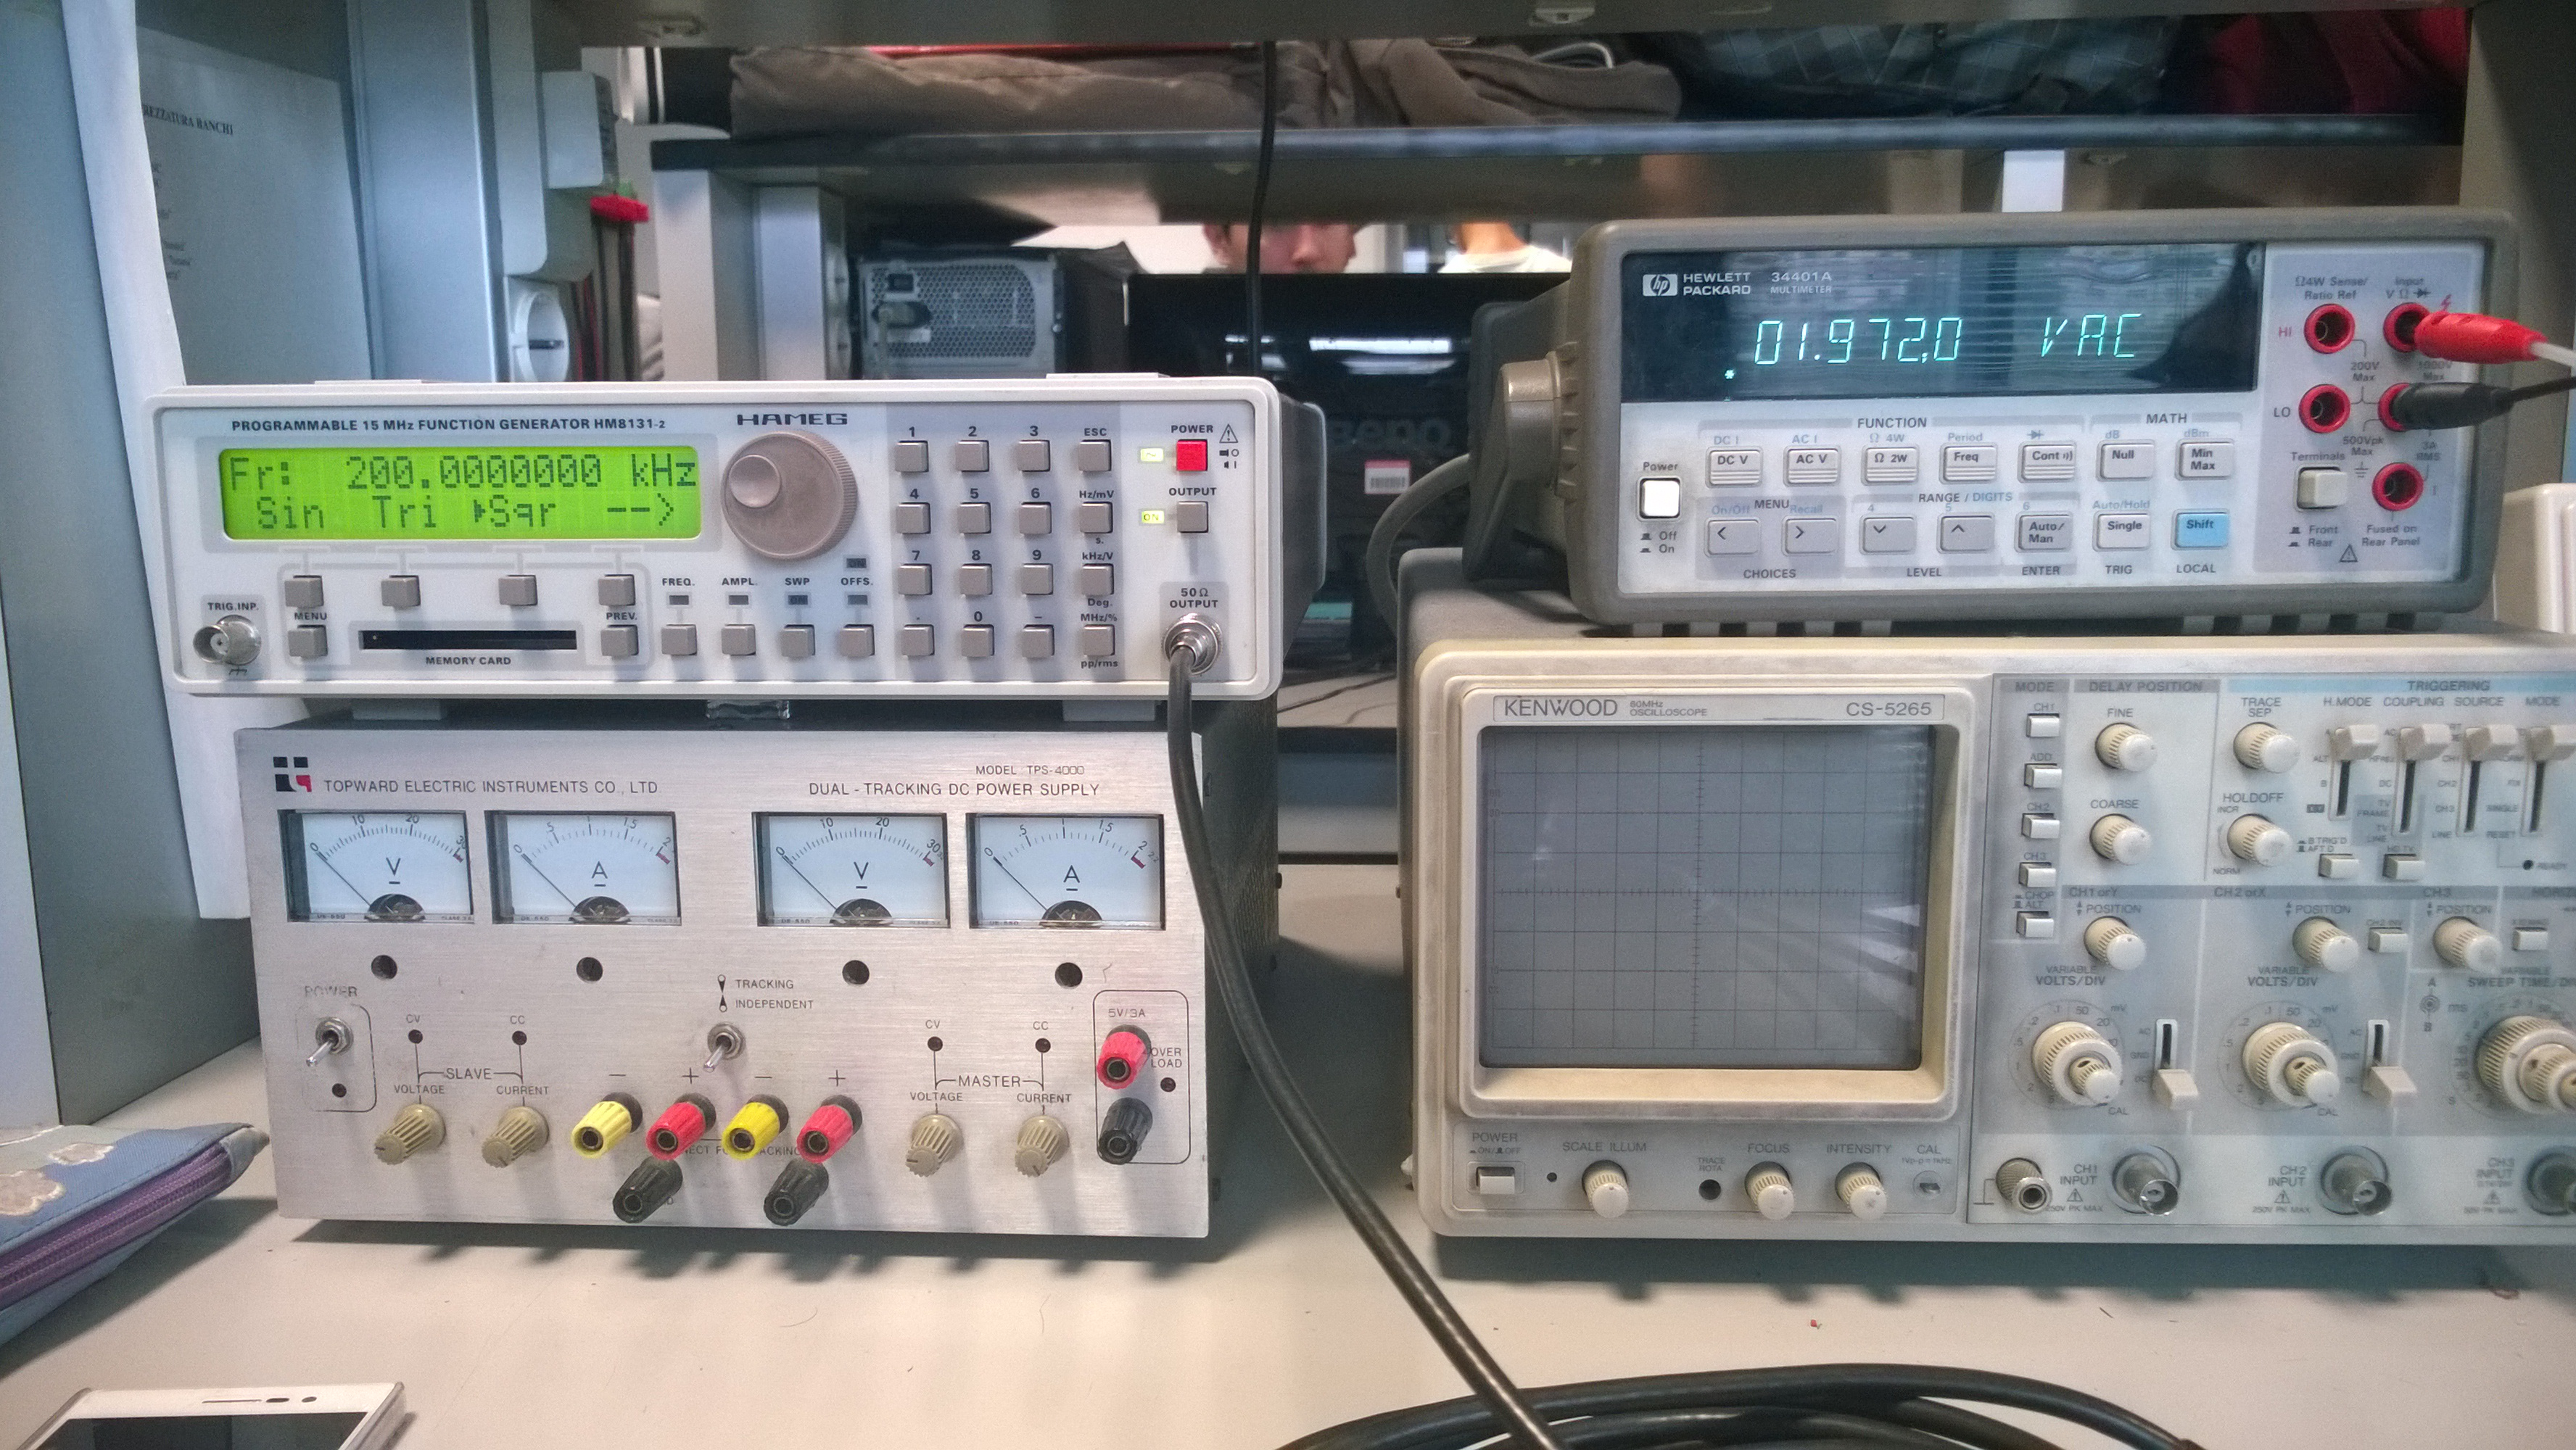
\includegraphics[scale=0.08]{foto/foto1.jpg}
\end{figure}

Si ottiene: \[V_{b1}=1,972 \pm 5,77\cdot10^{-5} V\]
\item Collegando in serie al generatore una resistenza di carico \(R_L=100\Omega\)  (come illustrato nella foto sottostante) si ottiene una tensione di uscita pari a: \(V_{b2}=1,294\pm1,53\cdot10^{-4} V\)
      \end{itemize}

\item []\textbf{B. Misura dei parametri del cavo}
  \begin{itemize}
    \item  Si è provato a collegare il generatore al cavo coassiale, con estremo aperto, in due modi differenti: con e senza basetta (come illustrato sotto).   

\begin{figure}[H]
\centering
  \minipage{0,4\textwidth}
    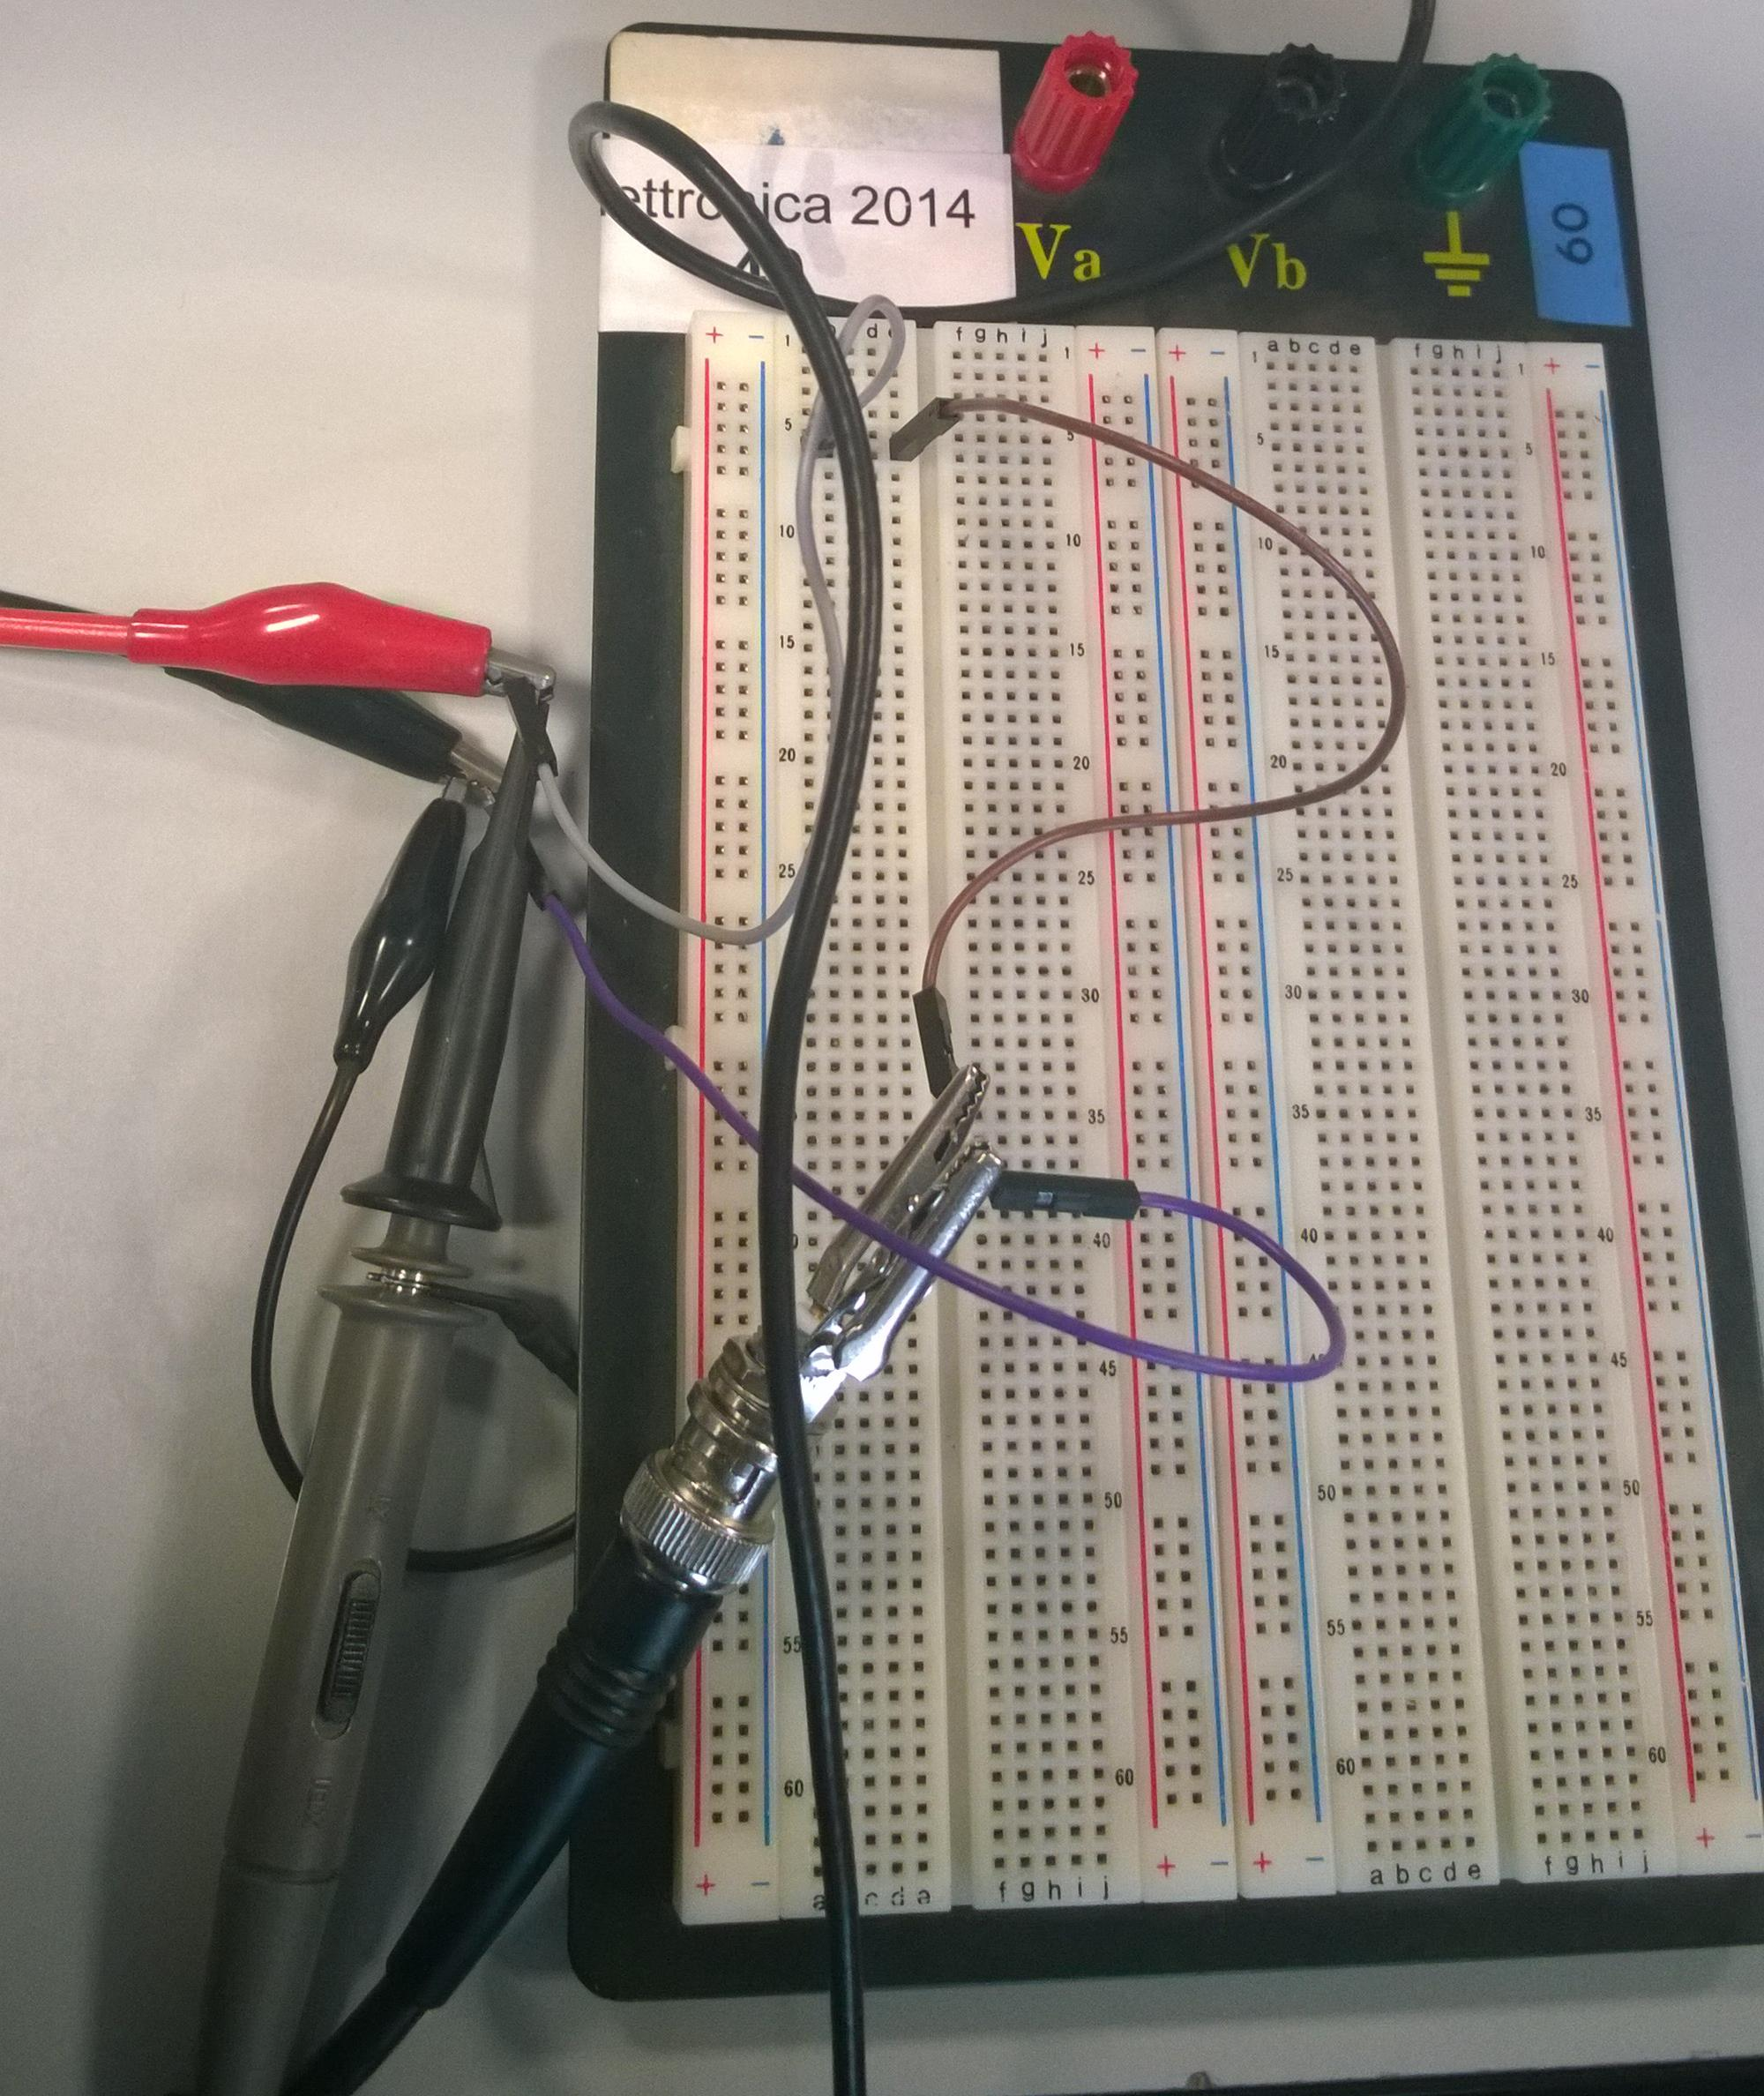
\includegraphics[scale=0.08]{foto/foto8.jpg}
  \endminipage
  \minipage{0,5\textwidth}
    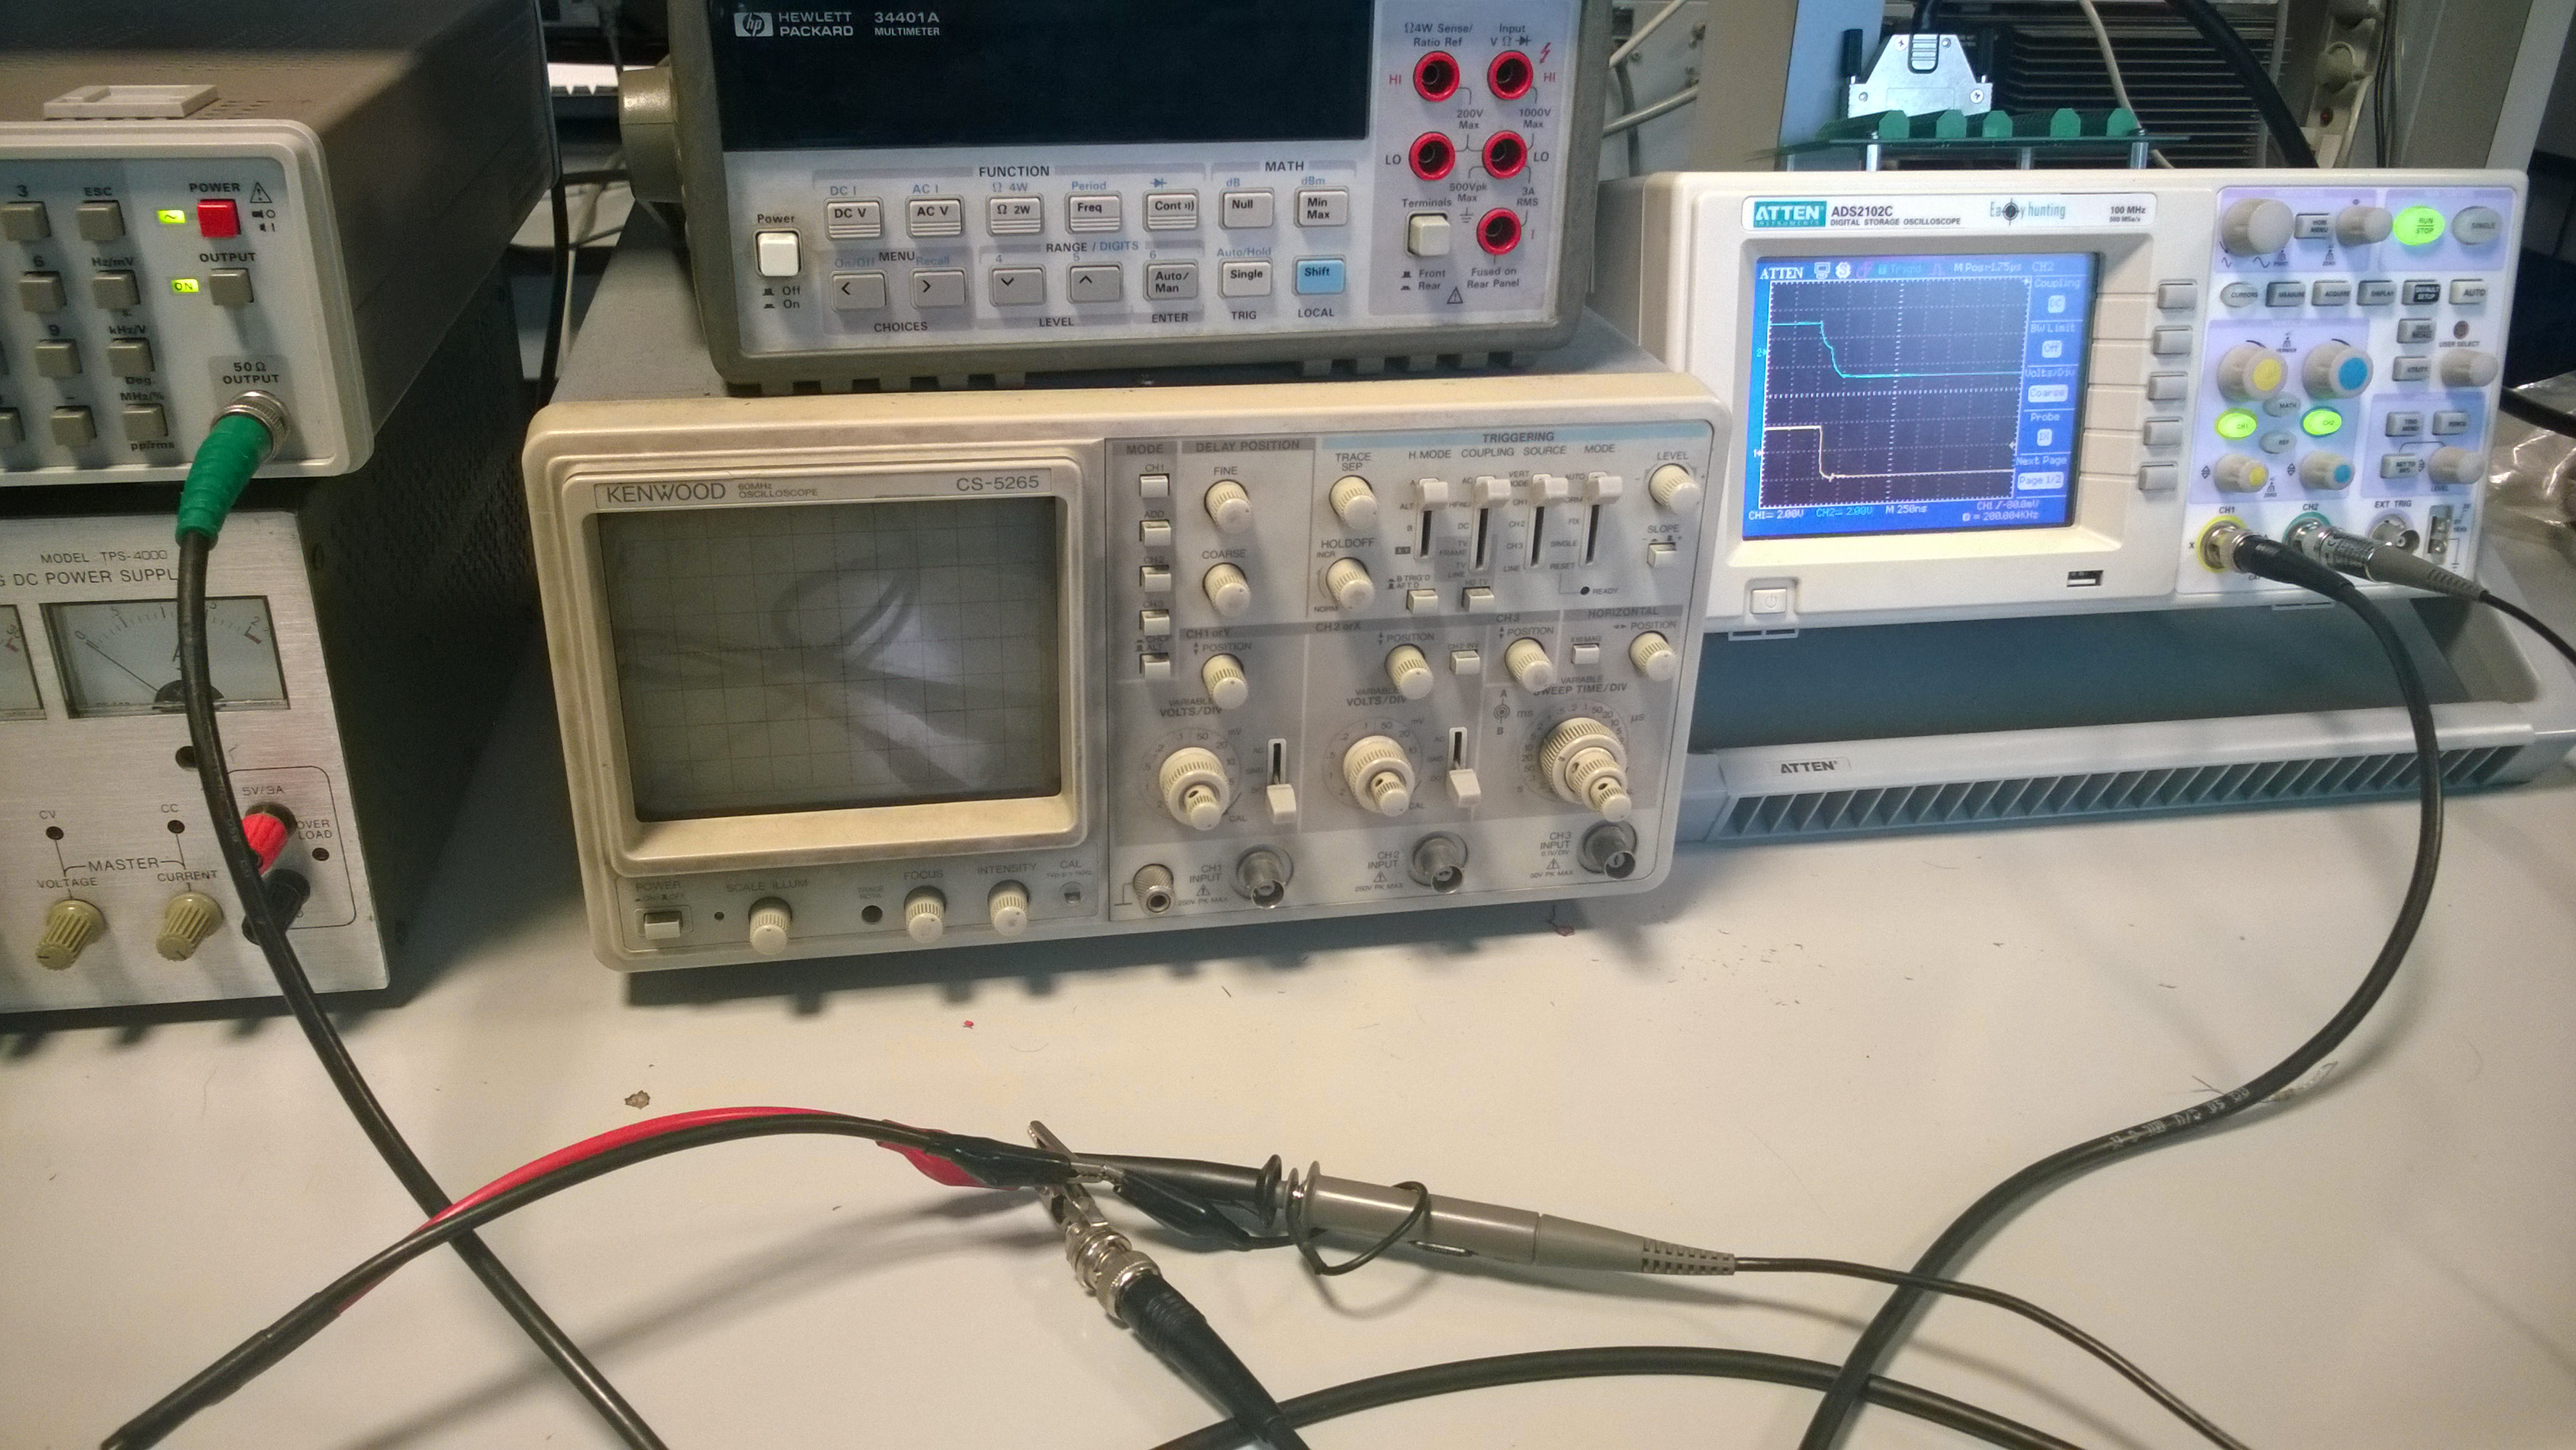
\includegraphics[scale=0.07]{foto/foto6.jpg}
  \endminipage
\end{figure}

Tramite l'oscilloscopio si osserva che il segnale blu è quello che si ottiene sul lato del generatore come somma di onda progressiva e onda riflessa (vedi i gradini);
il segnale giallo invece rappresenta la forma d'onda sull'altro estremo della linea di trasmissione.

\begin{figure}[!h]
\centering
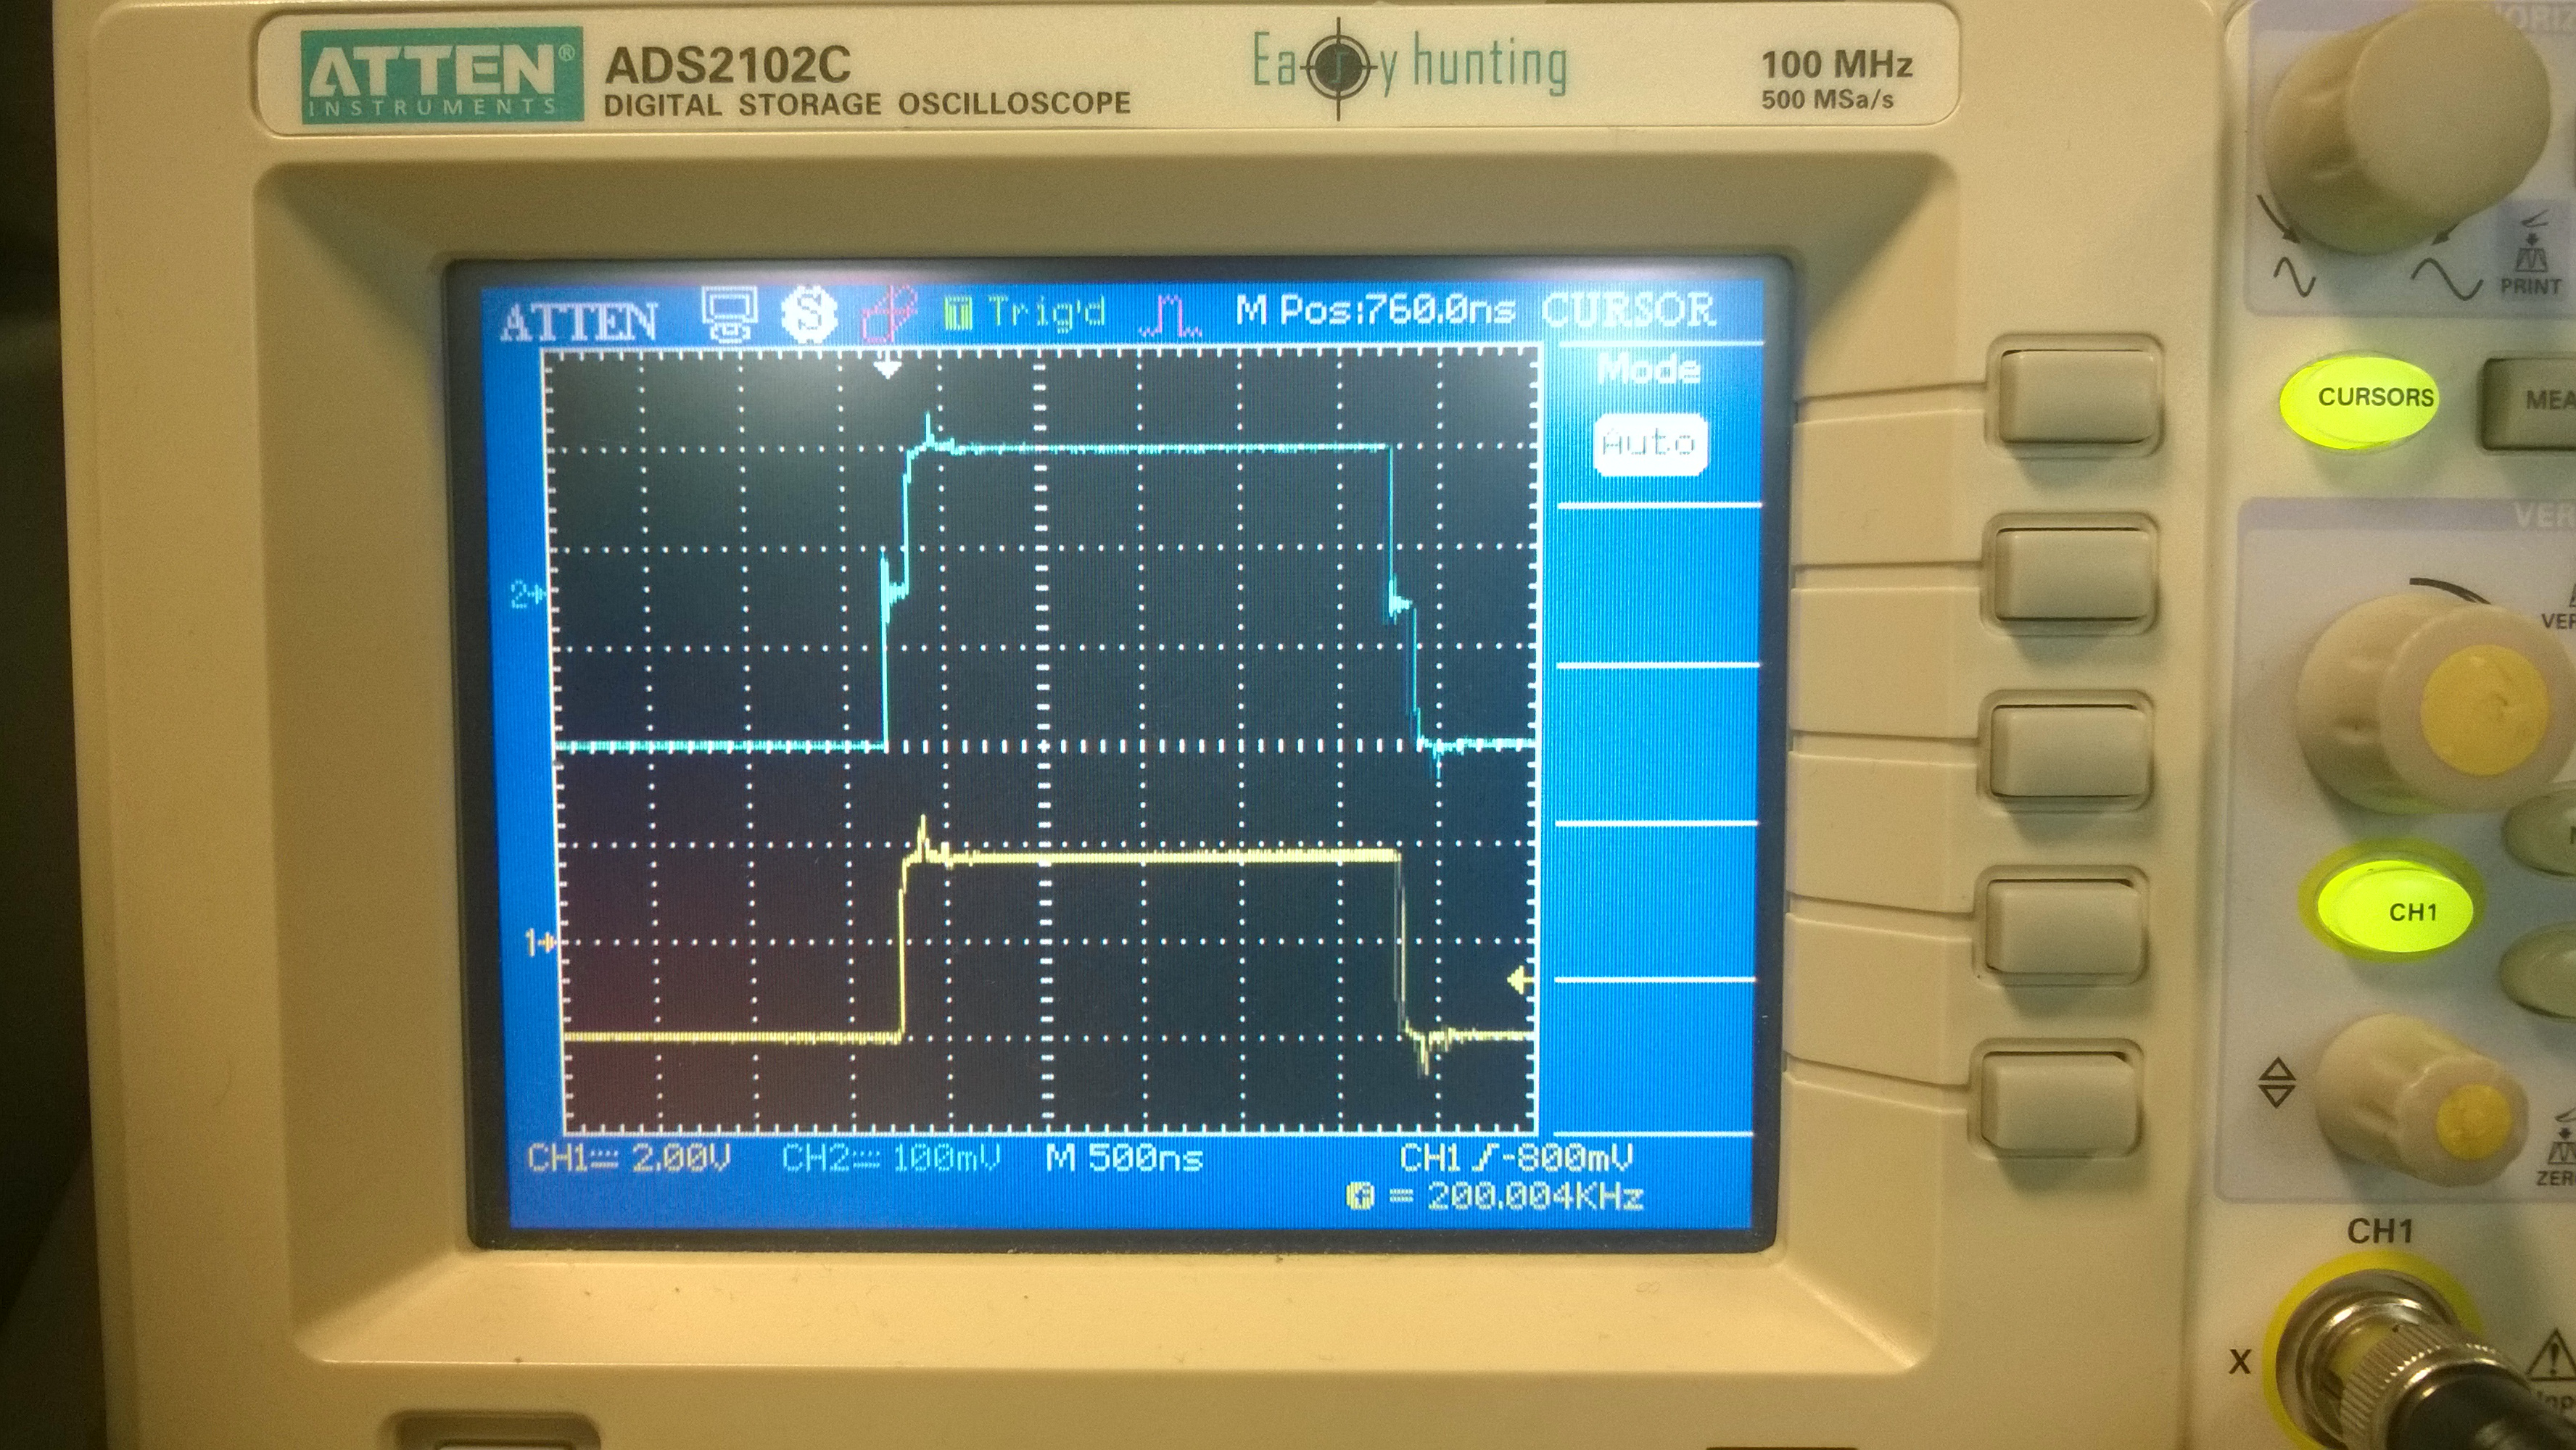
\includegraphics[scale=0.07]{foto/foto11.jpg}
\end{figure}

Dal ritardo di propagazione tra le due onde (\(\Delta T\)), trovato con l'ausilio dei cursori (come illustrato in foto), e dalla velocità di propagazione U (pari, nel caso di cavo RG58. a 0,66 c) si è calcolata la lunghezza del cavo coassiale: \[l=0,66c \cdot \Delta T=0,66c\cdot56ns=11,1 m\]

\begin{figure}[h]
\centering
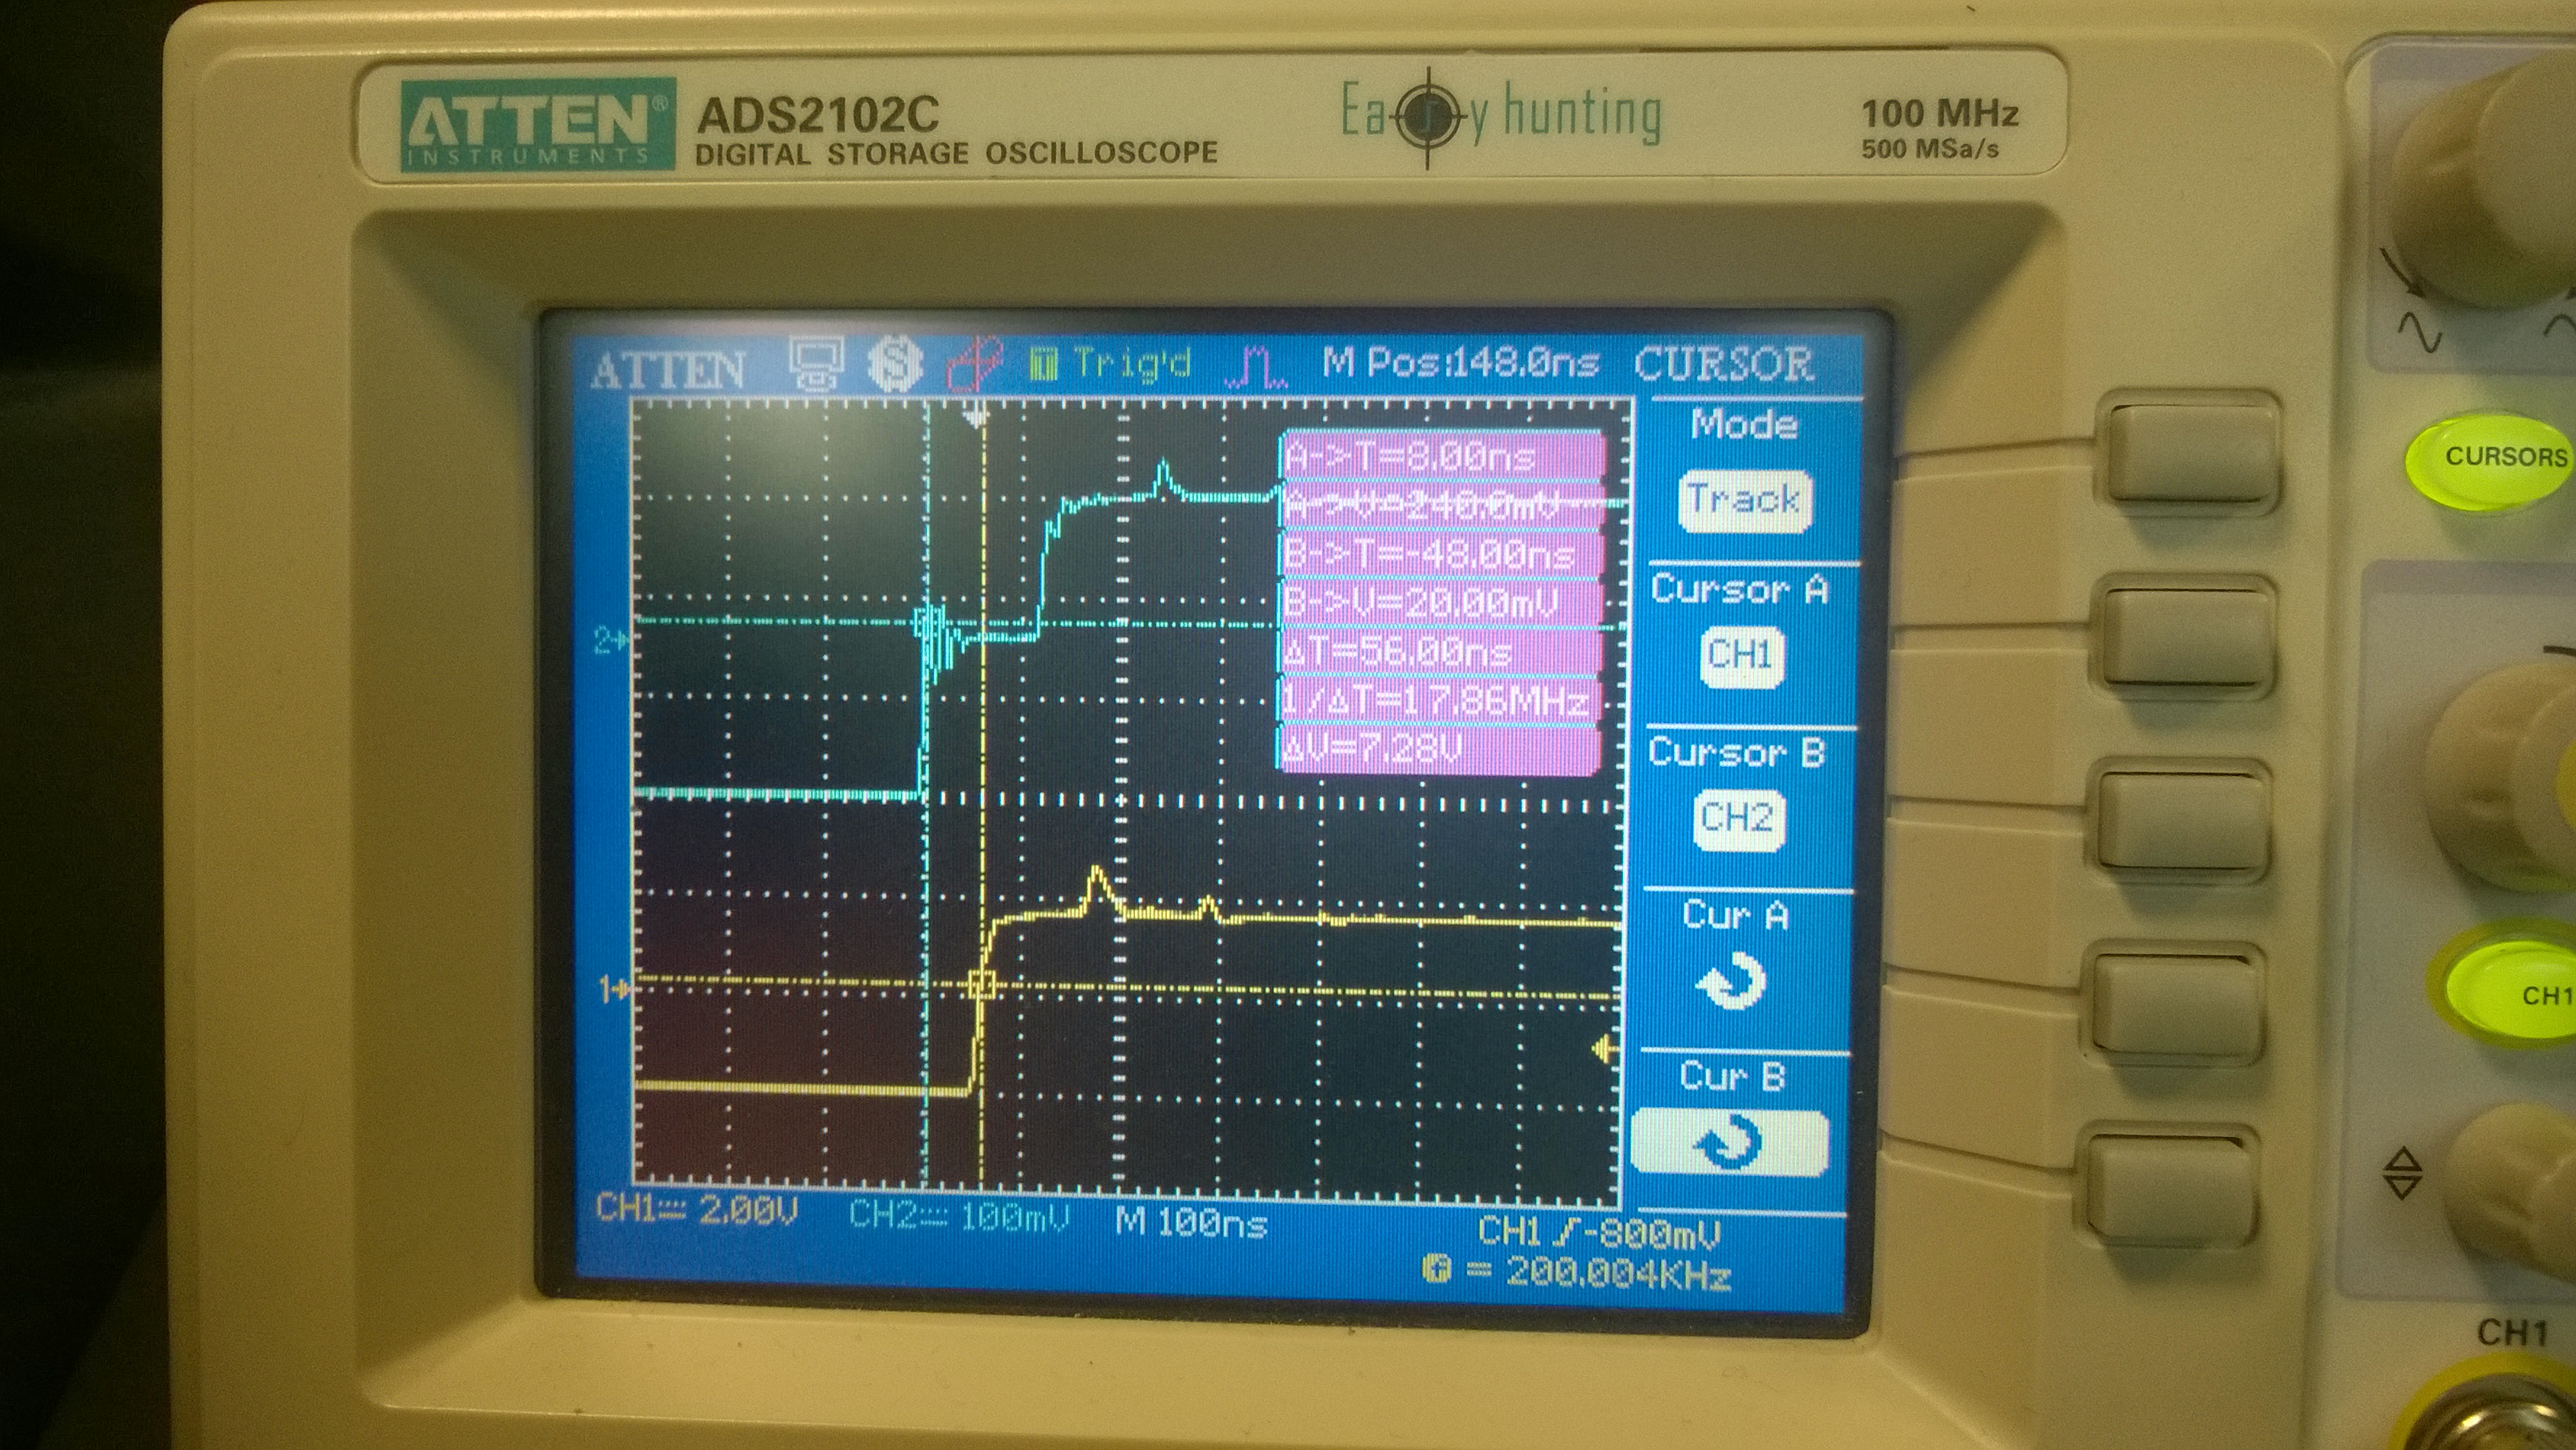
\includegraphics[scale=0.07]{foto/foto12.jpg}
\end{figure}

\item  Si aggiunge in terminazione una resistenza di \(50\Omega\) ottenuta come parallelo di due resistenze da \(100\Omega\). Sull'oscilloscopio si osserva l'assenza di gradini e quindi di riflessioni poichè il carico risulta adattato (\(R_T=Z_\infty=50\Omega\) ).

\begin{figure}[h]
\centering
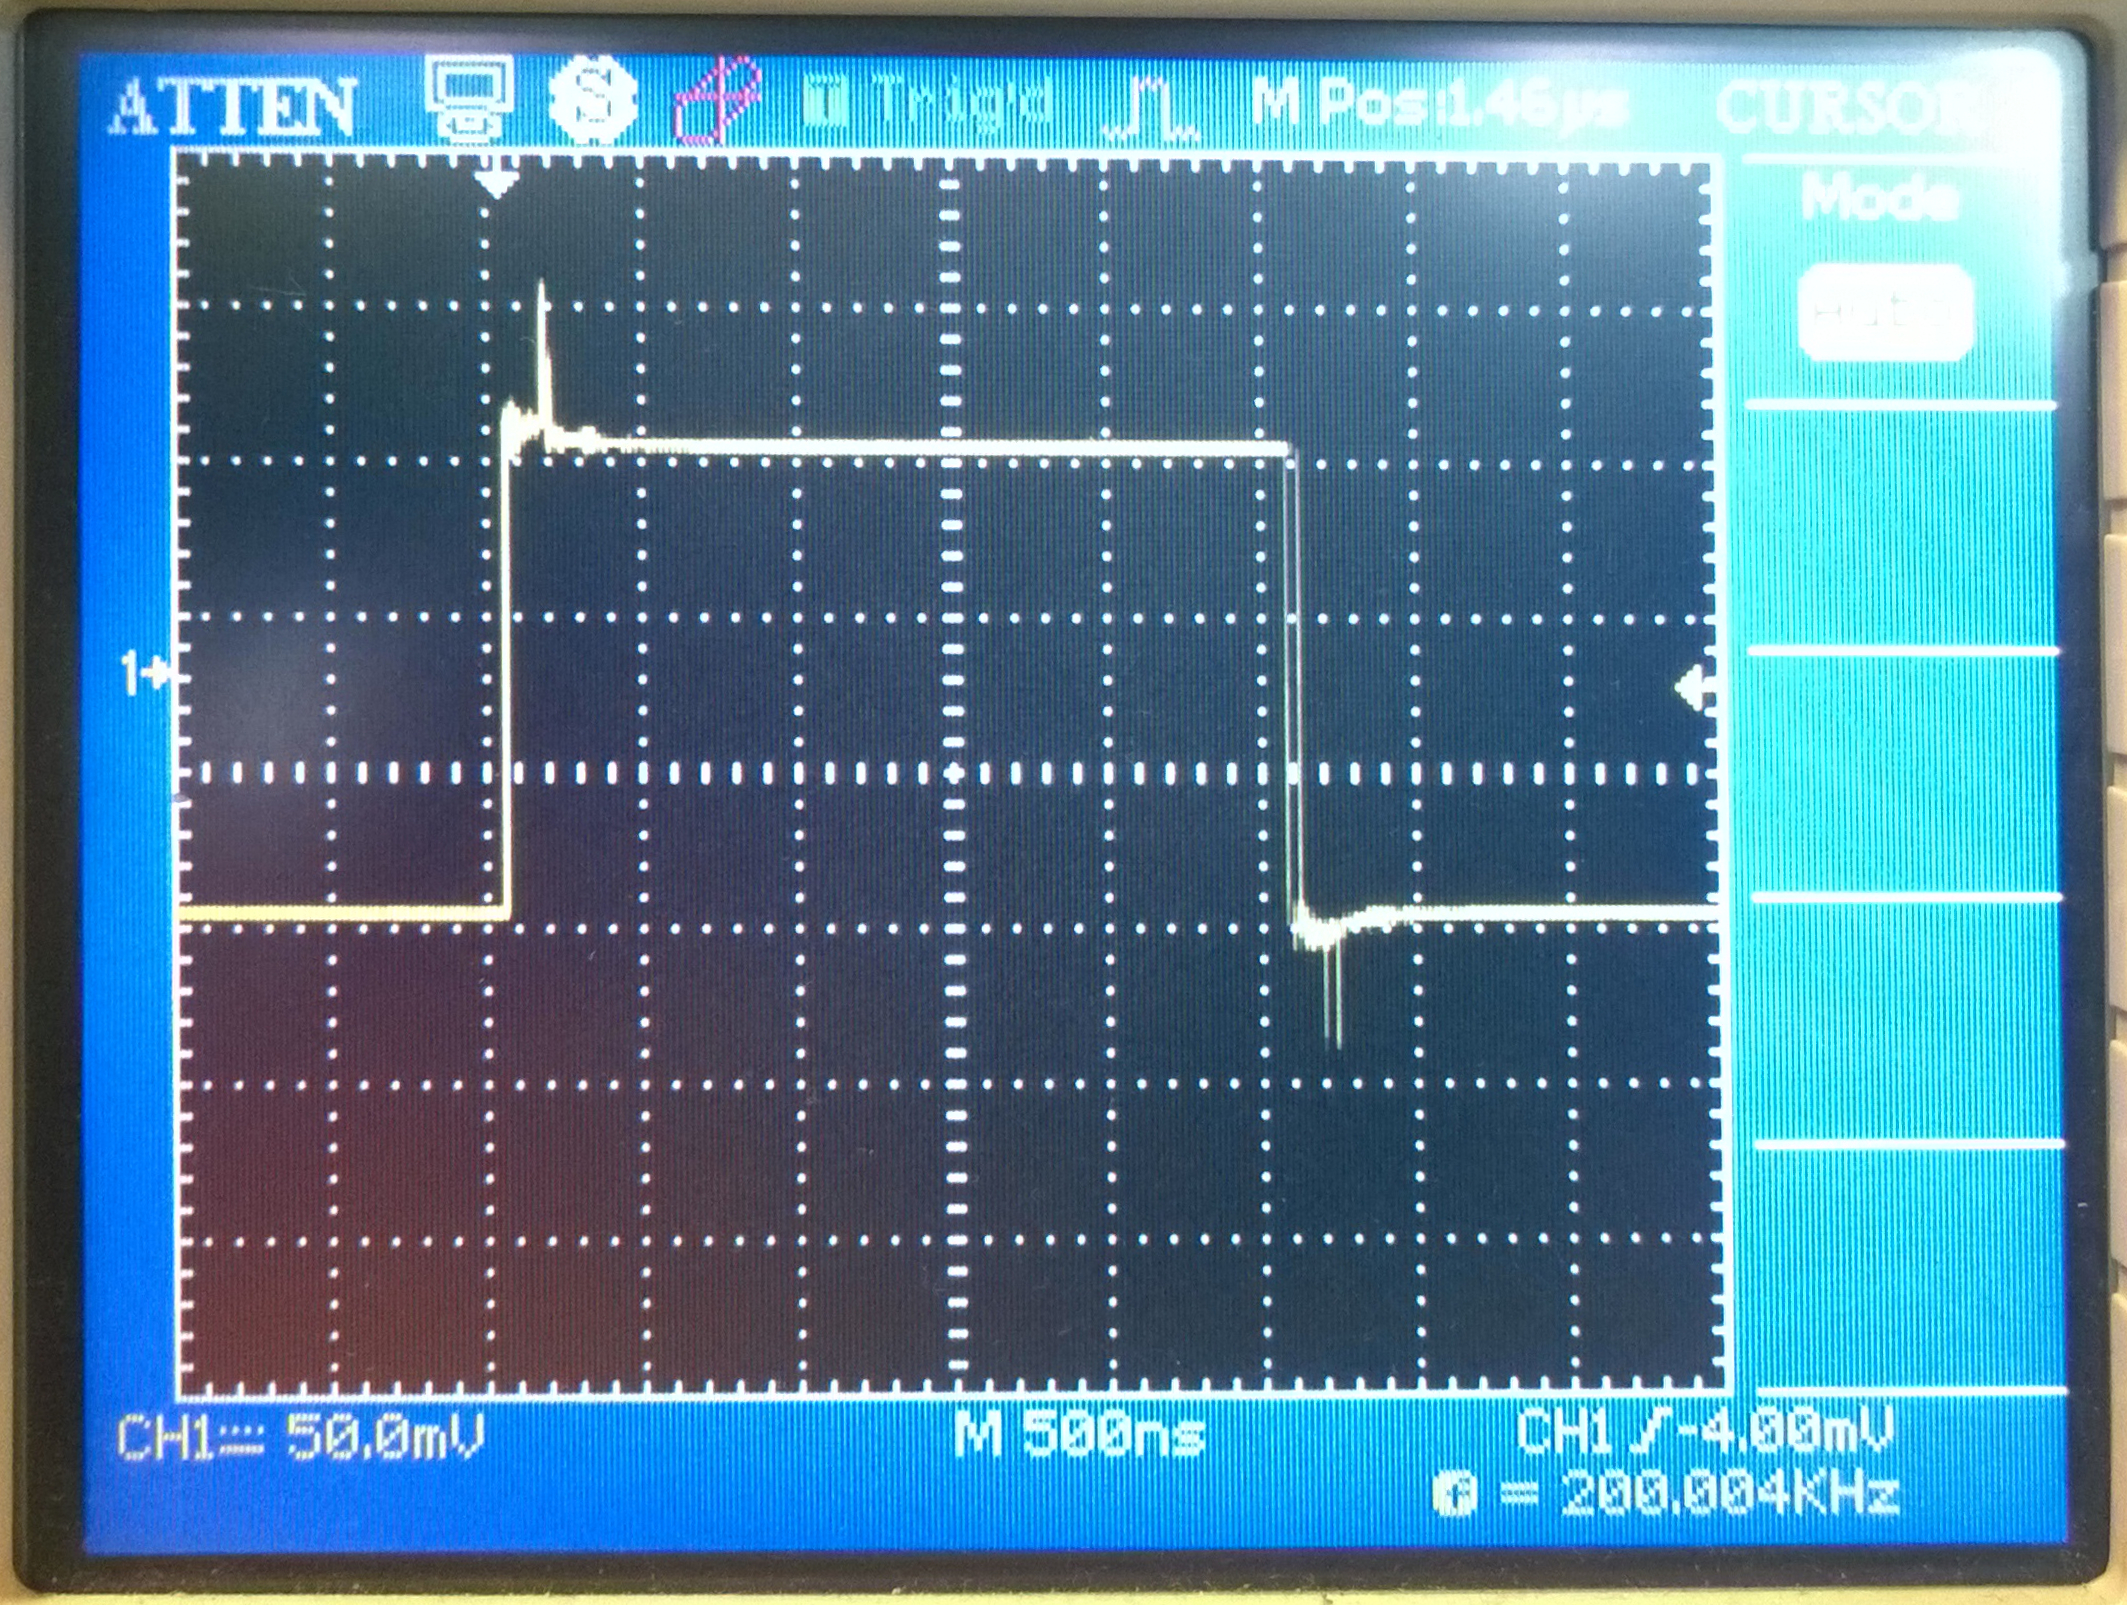
\includegraphics[scale=0.07]{foto/foto13.jpg}
\end{figure}

  \end{itemize}


\item []\textbf{C. Disadattamento lato driver e lato terminazione}
  \begin{itemize}
    \item Si collega una resistenza Rs (220 omh) in serie tra generatore e linea, in modo da lasciare aperta la linea all’estremo remoto, in questo modo il coefficiente \(\Gamma_g\) vale 1.

\begin{figure}[h]
\centering
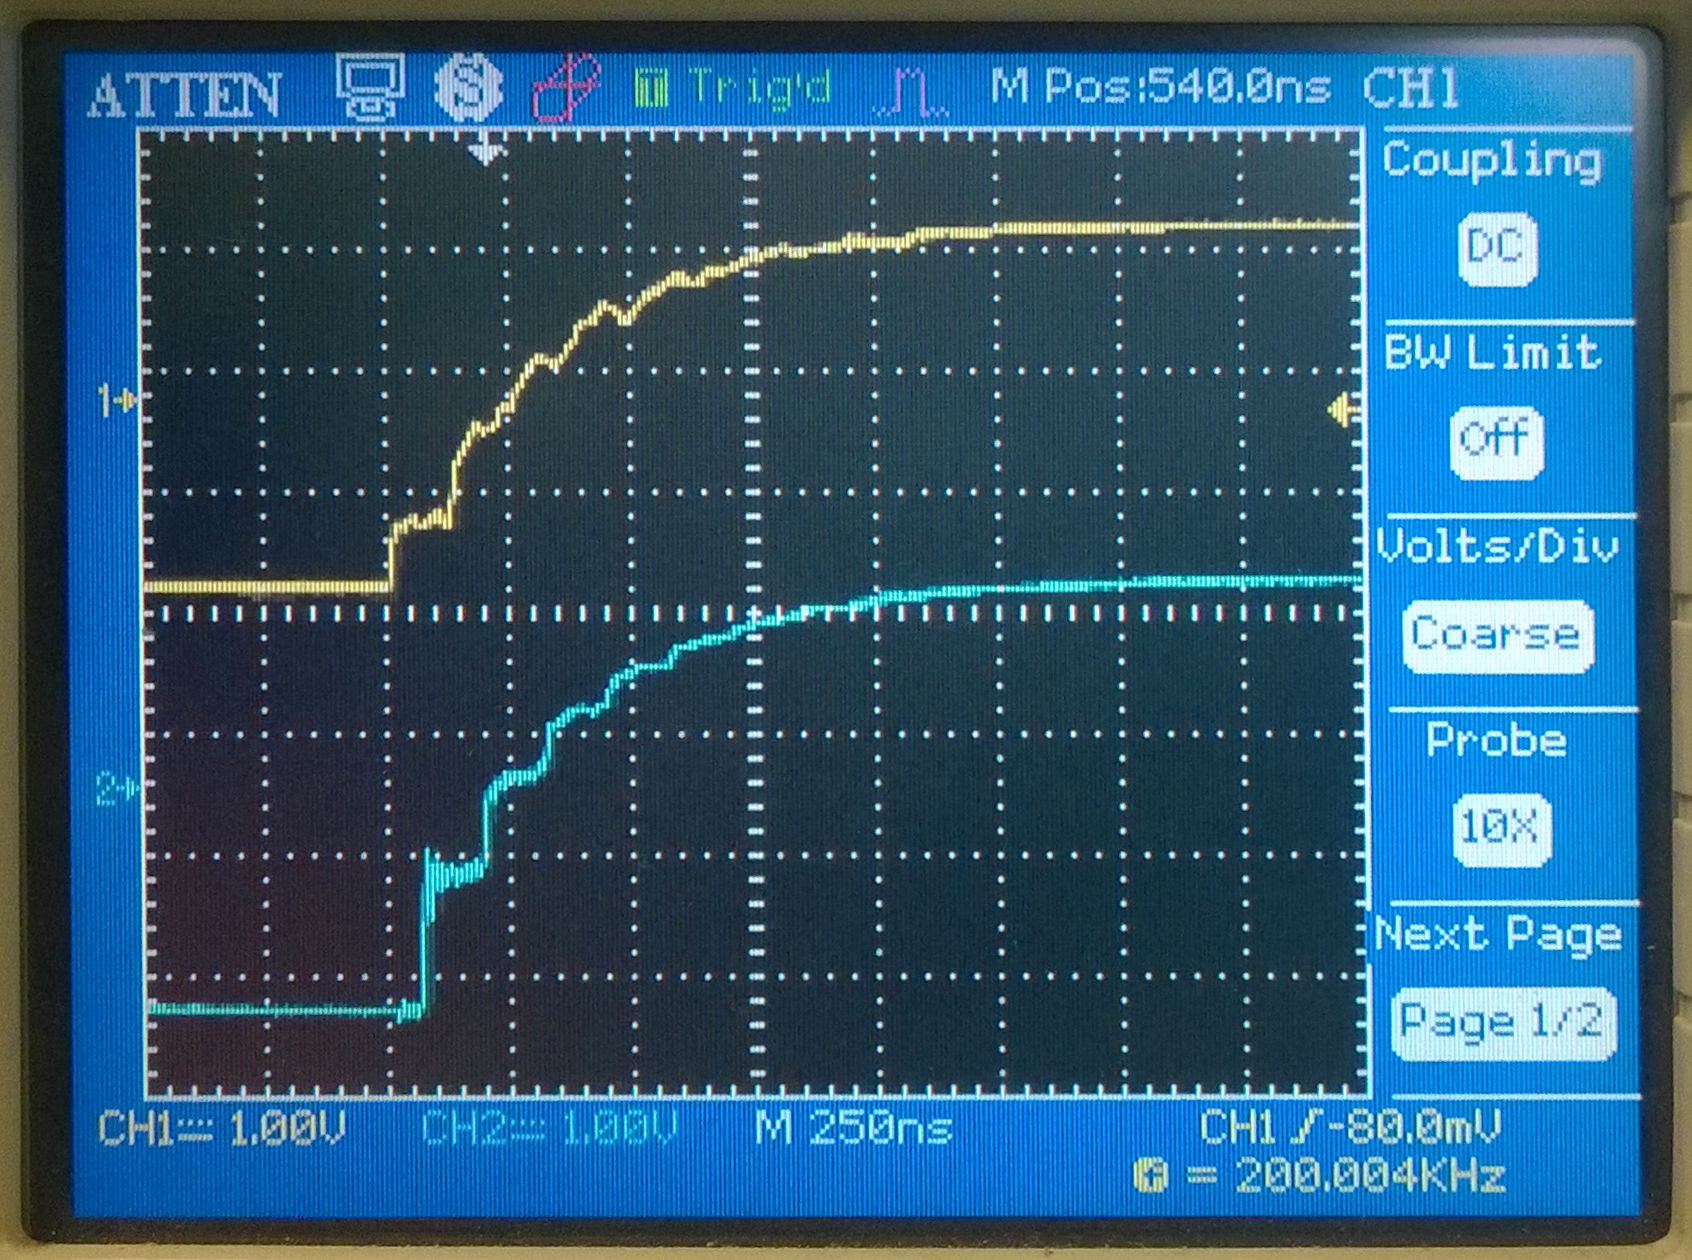
\includegraphics[scale=0.07]{foto/foto14.jpg}
\end{figure}

Si calcola il valore del coefficiente gamma lato generatore applicando la formula: 
\(\Gamma _g=\tfrac{R_g-Z_\infty}{R_g+Z_\infty}= 0,68\)

con \(R_g=R_0+R_s=(50+220)\Omega=270\Omega\)

Si confronta il risultato teorico con quello ottenuto misurando l’ampiezza dei gradini delle due forme d’onda.
\begin{center}
 \begin{tabular}{|r|l|l|l|l|}
     \hline
     \multicolumn{3}{|c|}{\(U (mV)\)} \\
     \hline
     \(502\) & \(500\) & \(504\)\\
     \hline
   \end{tabular} \\ \\
\[U_{medio}=502 \pm 1,15 mV\]

\begin{tabular}{|r|l|l|l|l|}
     \hline
     \multicolumn{3}{|c|}{\(v (V)\)} \\
     \hline
     \(1,33\) & \(1,34\) & \(1,31\)\\
     \hline
   \end{tabular} \\ \\
\[v_{medio}=1,33 \pm 0,01 V\]
\end{center}
Applicando il diagramma a traliccio si ha:
\[\Gamma_g = \tfrac{v-2U}{U} = 0,66 \pm 0,03 \]
\item Si ripete la misura ponendo una resistenza da 22 omh in parallelo sull’uscita del generatore in modo da avere una misura con resistenza equivalente del generatore più bassa dell’impedenza caratteristica.

\begin{figure}[h]
\centering
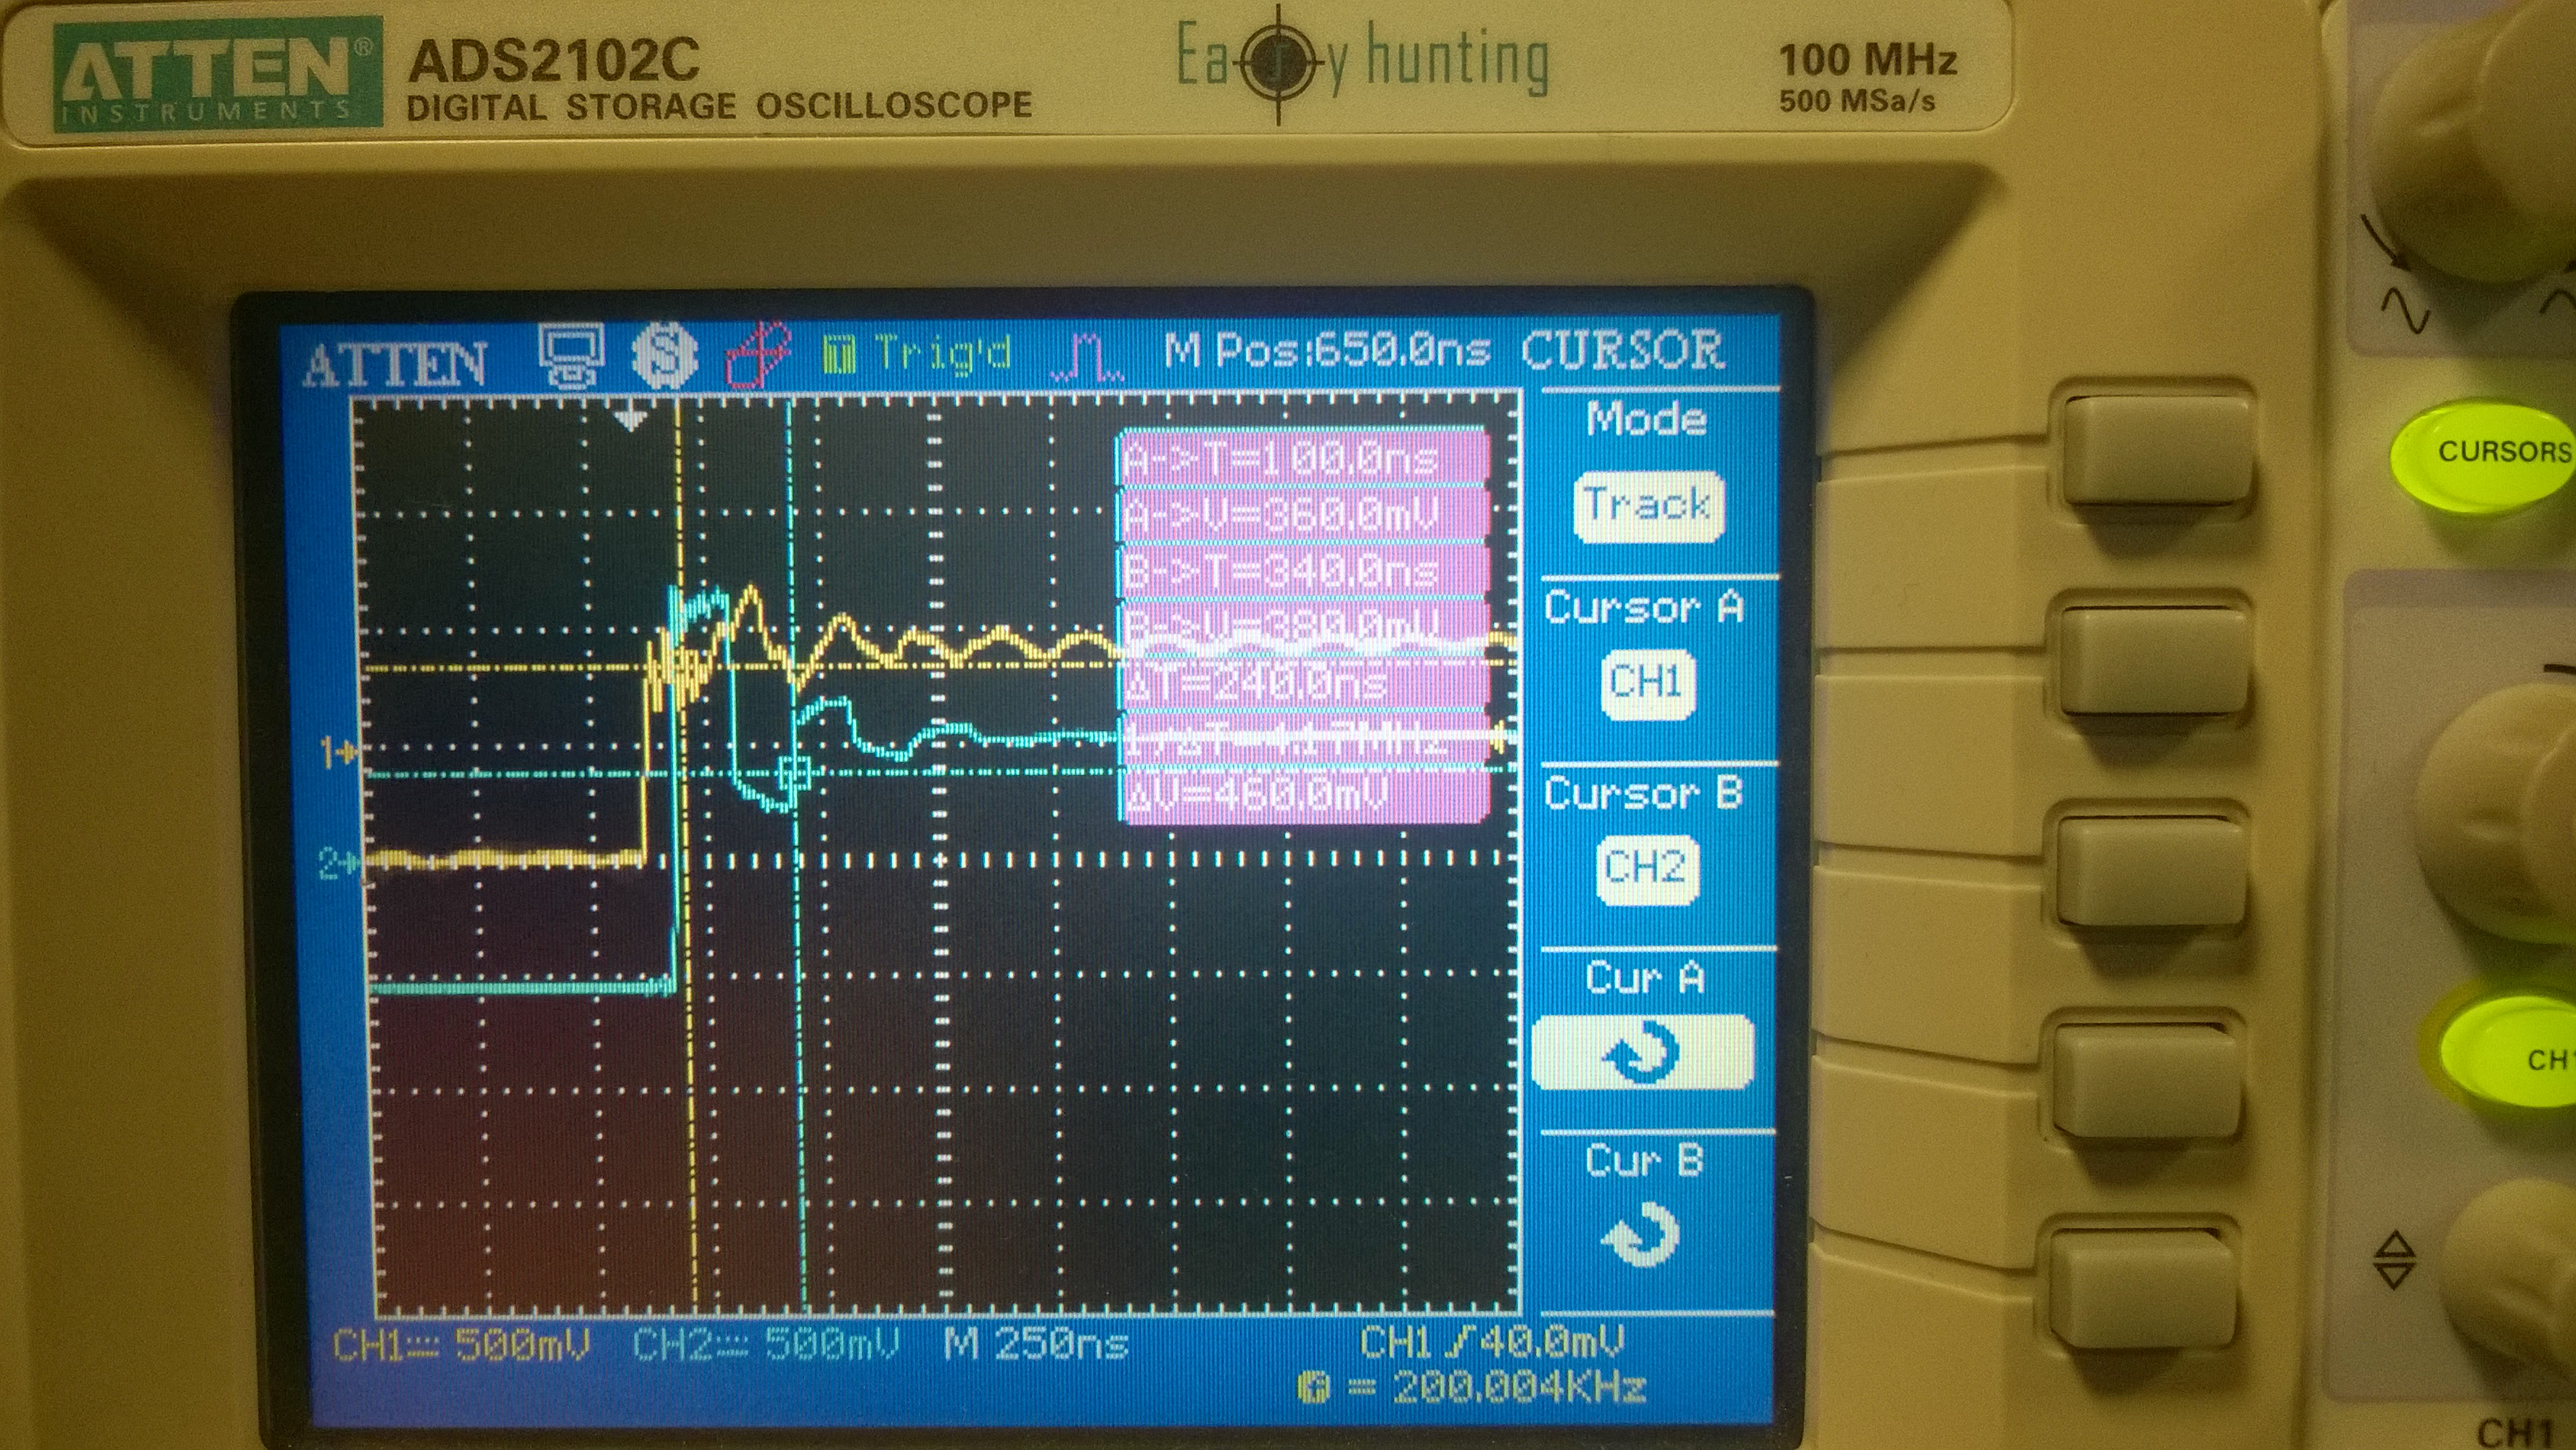
\includegraphics[scale=0.07]{foto/foto15.jpg}
\end{figure}

Si osservano delle oscillazioni dovute al fatto che il coefficiente di riflessione lato generatore gamma g è negativo.

Si calcola il valore del coefficiente gamma g applicando la formula: 
\(\Gamma _g=\tfrac{R_g-Z_\infty}{R_g+Z_\infty}= -0,53\)

Con \(R_g=R_0\parallel R_s= (50\parallel 22)\Omega = 15,28 \Omega\)

Si confronta il risultato teorico con quello ottenuto misurando l’ampiezza dei gradini delle due forme d’onda.
\begin{center}
 \begin{tabular}{|r|l|l|l|l|}
     \hline
     \multicolumn{3}{|c|}{\(U (mV)\)} \\
     \hline
     \(882\) & \(885\) & \(894\)\\
     \hline
   \end{tabular} \\ \\
\[U_{medio}=887 \pm 3,60 mV\]

\begin{tabular}{|r|l|l|l|l|}
     \hline
     \multicolumn{3}{|c|}{\(v (V)\)} \\
     \hline
     \(1,26\) & \(1,34\) & \(1,31\)\\
     \hline
   \end{tabular} \\ \\
\[v_{medio}=1,30 \pm 0,02 V\]
\end{center}
Applicando il diagramma a traliccio si ha:  
\[\Gamma_g = \tfrac{v-2U}{U} = -0,53 \pm 0,02\]
  \end{itemize}
\item []\textbf{D. Carico capacitivo} \\
  Si collega un condensatore \(C_T= 1 nF\) all’estremo remoto del cavo, e si verificano le forme d’onda agli estremi del cavo, in particolare quando il gradino raggiunge l’estremo remoto, il condensatore può essere considerato un corto circuito
 (\(\Gamma _T= -1\)), mentre a transitorio esaurito diventa un circuito aperto (\(\Gamma _T= 1\))

\begin{figure}[H]
\centering
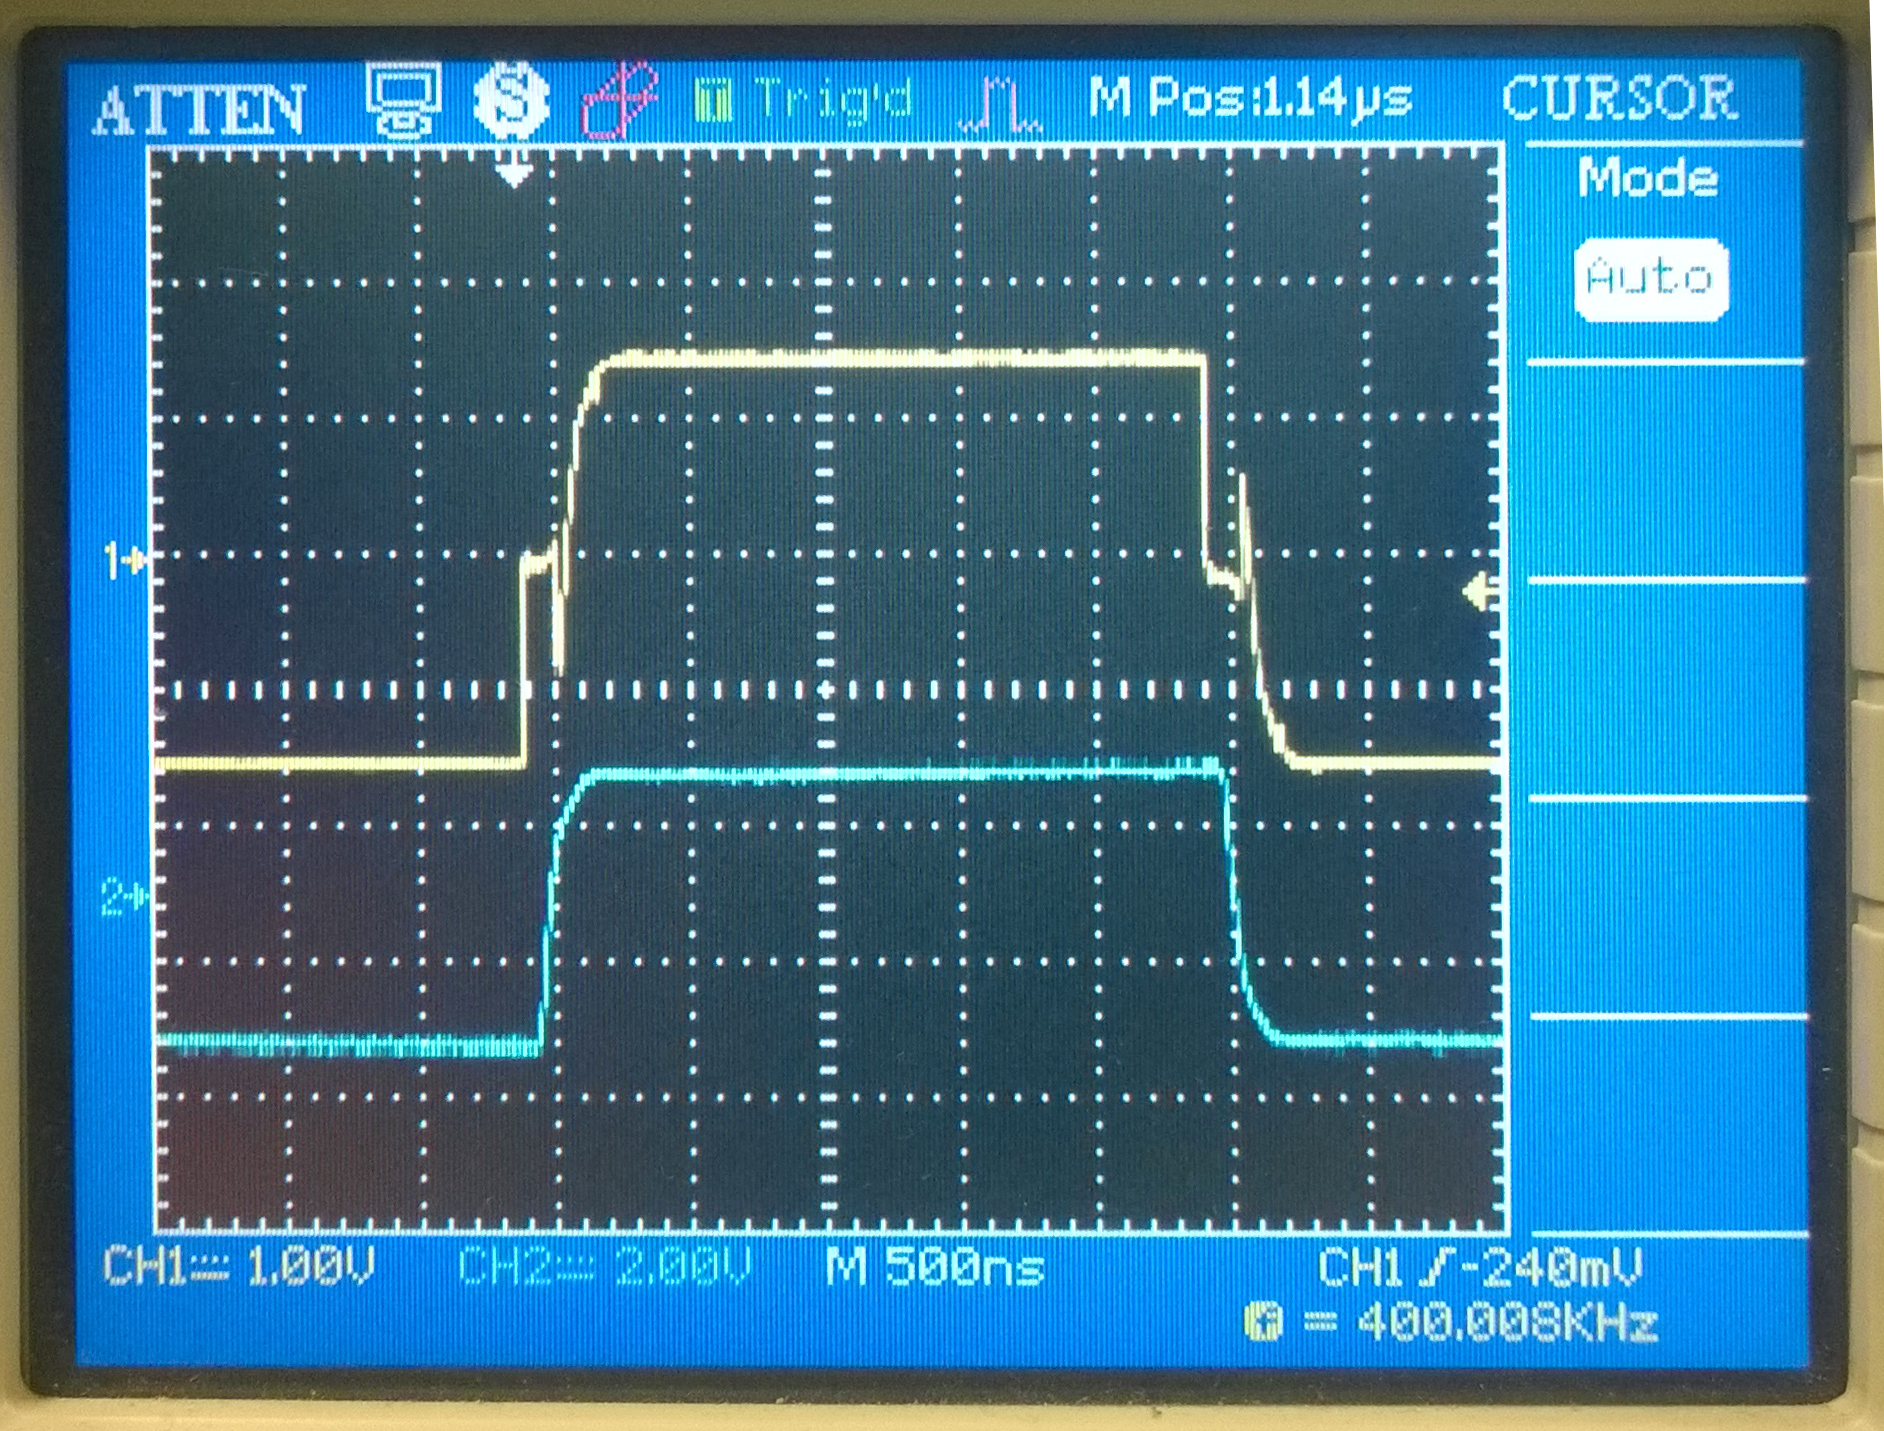
\includegraphics[scale=0.07]{foto/foto16.jpg}
\end{figure}

\item []\textbf{E. Riflettometria nel dominio del tempo} \\
  Si misura la lunghezza del cavo attraverso la misura dell’ampiezza del gradino intermedio all’estremo vicino attraverso la formula: 
\[2l=0,66c\cdot2t_p=0,66\cdot 3 \cdot 10^8 \cdot 112 ns = 22,2 m\]

\begin{figure}[H]
\centering
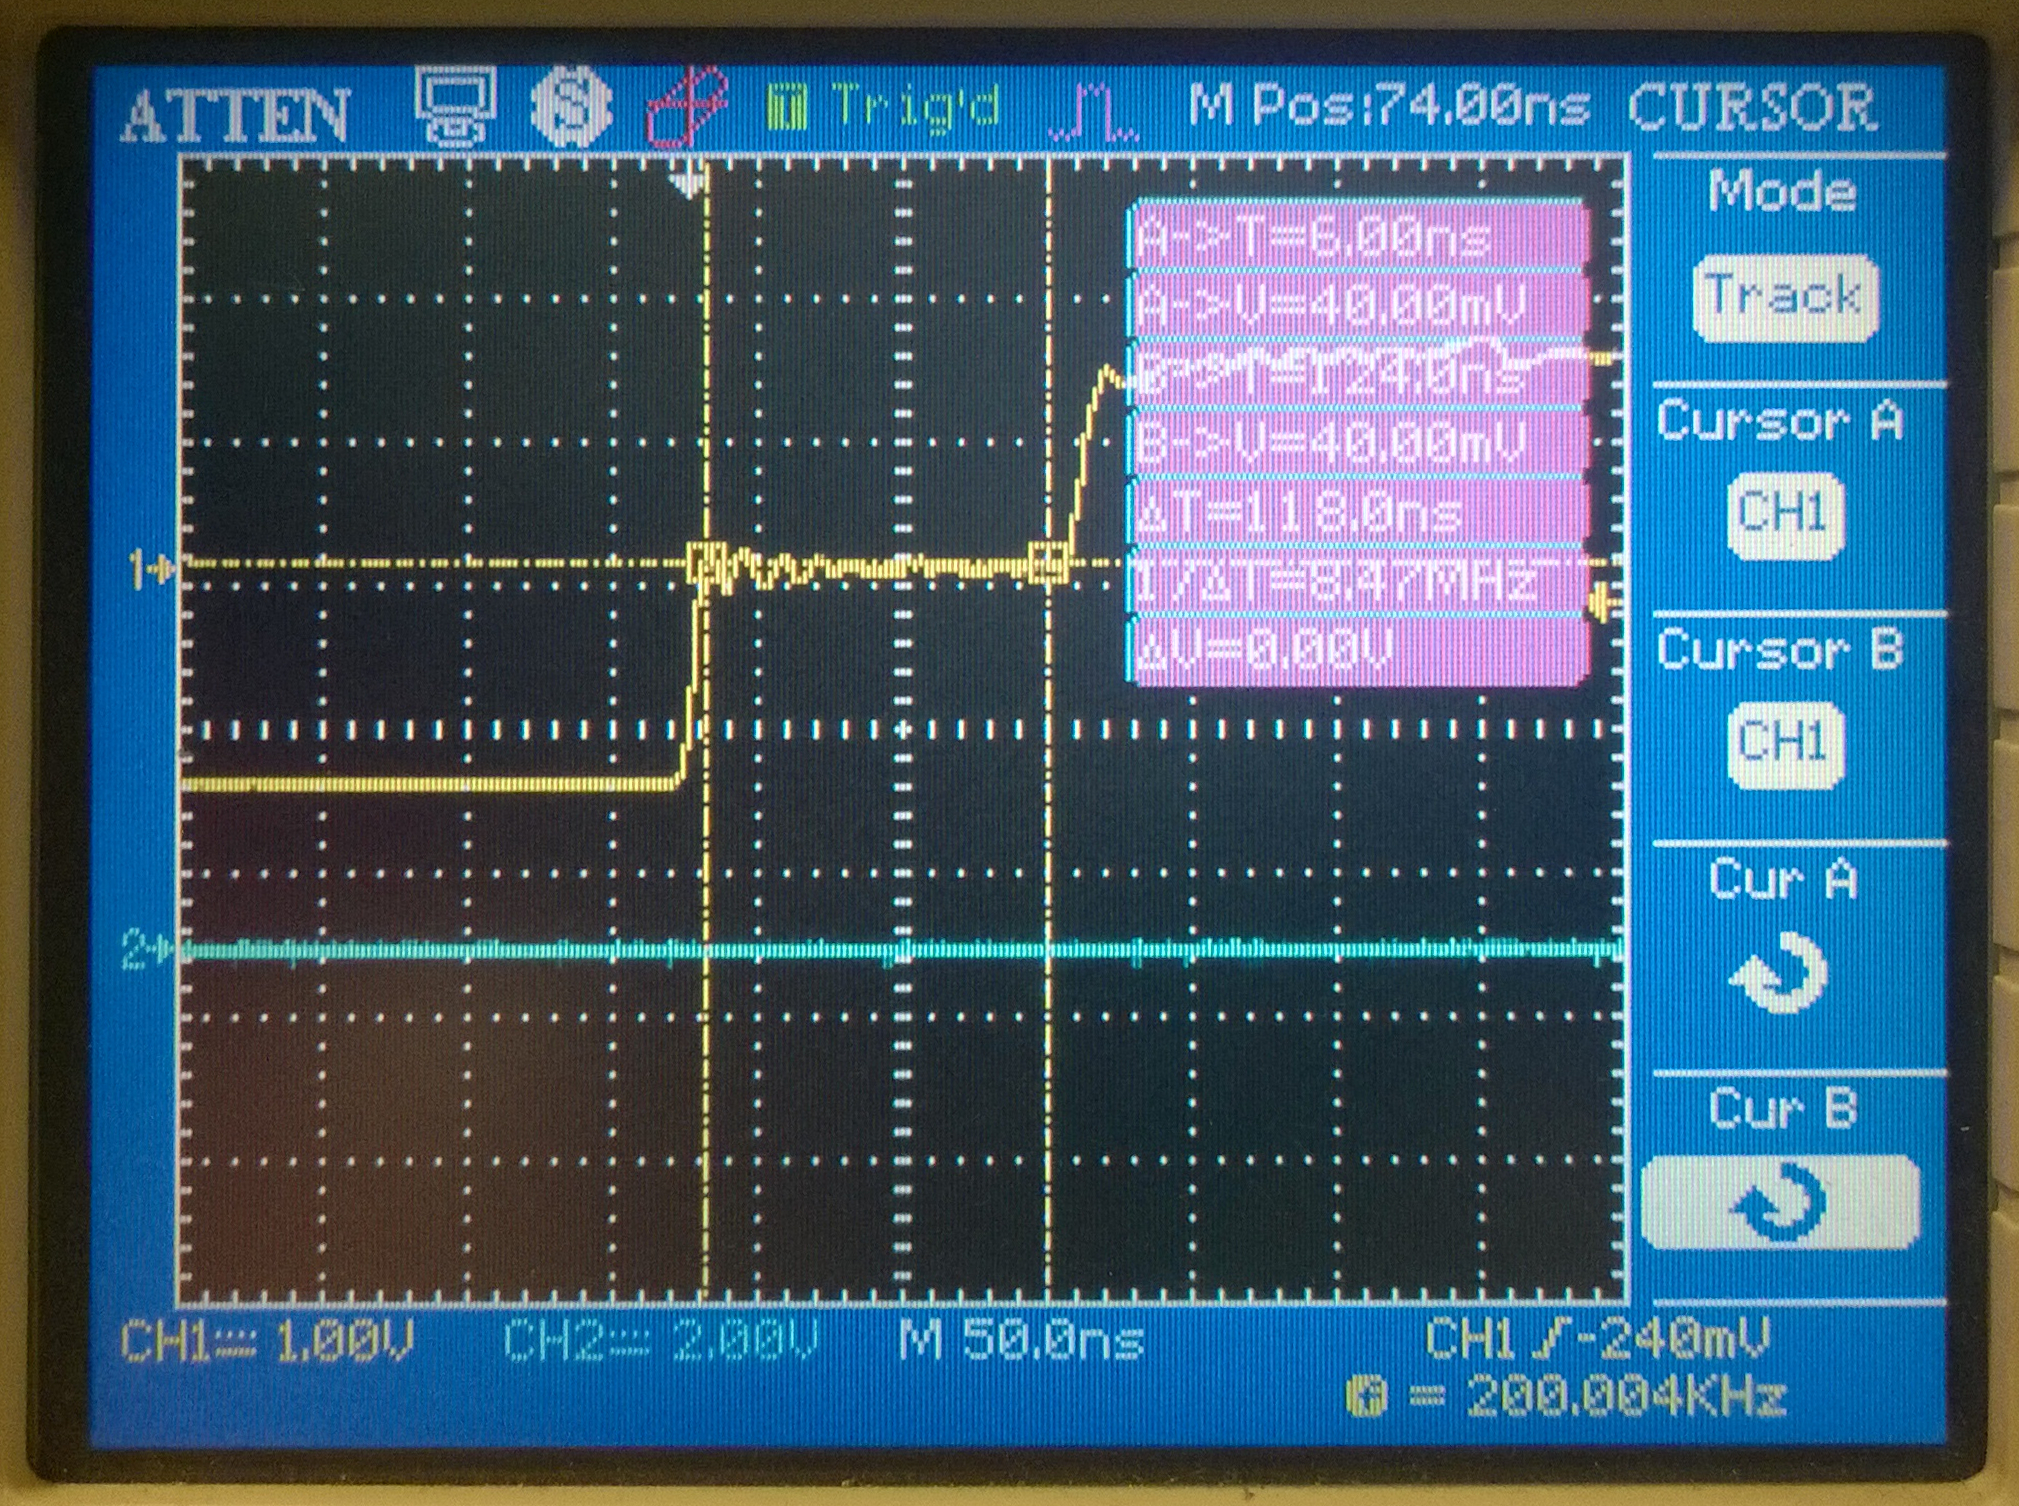
\includegraphics[scale=0.07]{foto/foto18.jpg}
\end{figure}

\end{itemize}

\LaTeX
\end{document}